%----------------------------------------------------------------------------------------
% Preambulo y Configuración
%----------------------------------------------------------------------------------------

\documentclass[
    11pt,
    spanish,
    singlespacing,
    parskip,
    headsepline,
    bookmarks=true,
    unicode=true,
    pdftoolbar=true,
    pdfmenubar=true,
    pdffitwindow=false,
    colorlinks=true,
    linkcolor=blue,
    citecolor=blue,
    urlcolor=blue
]{MastersDoctoralThesis}

\usepackage{float}
\usepackage{rotating}
\usepackage{pdflscape}

\usepackage[utf8]{inputenc} % Codificación de entrada UTF-8
\usepackage[T1]{fontenc}    % Codificación de salida para caracteres especiales
\usepackage{graphicx}       % Manejo de gráficos
\usepackage{eso-pic}        % Permite agregar fondos
\usepackage{hyperref}       % Manejo de hipervínculos y marcadores

% Redefinición de caracteres problemáticos en marcadores
\hypersetup{
    pdftitle={Título del Documento},
    pdfauthor={Autor del Documento},
    pdfkeywords={Sistemas Embebidos, Internet de las Cosas, Inteligencia Artificial},
    pdfstartview={FitH},
    unicode=true,
    colorlinks=true,
    linkcolor=blue,
    citecolor=blue,
    urlcolor=blue
}

\pdfstringdefDisableCommands{%
  \def\texttt#1{#1}%
  \def\textbf#1{#1}%
  \def\textit#1{#1}%
  \def\"{\"}%
  \def\~{~}%
  \def\'{'}%
  \def\^{}%
  \def\textunderscore{\_} % Manejo del subrayado en marcadores
}


% Definir comandos requeridos por la clase
\newcommand{\degreename}{Maestría en Ciencias} % Cambia según tu título
\newcommand{\univname}{Universidad Nacional de Ejemplo} % Cambia según tu universidad
\newcommand{\keywordnames}{Palabras clave:}
%----------------------------------------------------------------------------------------
% Documento Principal
%----------------------------------------------------------------------------------------

\begin{document}

% Configuración de la portada
\posgrado{Carrera / Maestría}
\keywords{Sistemas Embebidos, Internet de las Cosas, Inteligencia Artificial}

% Incluir la portada desde un archivo separado
%----------------------------------------------------------------------------------------
% PORTADA
%----------------------------------------------------------------------------------------
\begin{titlepage}
    % Fondo completo con el PDF que incluye la barra y el logo
    \AddToShipoutPictureBG*{\includegraphics[width=\paperwidth, height=\paperheight]{Figures/fondo.pdf}}

    % Contenido principal
    \begin{flushright}
        \setlength{\rightskip}{-2cm} % Ajusta la sangría derecha
        \vspace*{7.5cm} % Ajustar según la posición vertical deseada

        % Título
        {\fontfamily{phv}\bfseries\fontsize{33pt}{40pt}\selectfont
        Tester para amplificador óptico} \\[1.5cm]

        % Autor
        {\fontfamily{phv}\fontsize{20pt}{25pt}\selectfont
        Ing. Lucas Constantino} \\[1cm]

        % Carrera o Maestría (comentar o descomentar la línea correspondiente)
        {\fontfamily{phv}\fontsize{15pt}{20pt}\selectfont
        \textbf{Carrera de Especialización en Sistemas Embebidos}
        % \textbf{Carrera de Especialización en Internet de las Cosas} \\
        % \textbf{Carrera de Especialización en Inteligencia Artificial} \\
        % \textbf{Maestría en Sistemas Embebidos} \\
        % \textbf{Maestría en Internet de las Cosas} \\
        % \textbf{Maestría en Inteligencia Artificial Embebida} \\
        % \textbf{Maestría en Computación de Borde} \\
        % \textbf{Maestría en Inteligencia Artificial} \\
        } \\[2cm]

        % Director
        {\fontfamily{phv}\fontsize{11pt}{15pt}\selectfont
        \textbf{Director:} Dr. Ing. Alejandro Ghersin (FIUBA)} \\[1cm]

        % Jurados
        {\fontfamily{phv}\fontsize{11pt}{15pt}\selectfont
        \textbf{Jurados:}} \\[0.5cm]
        {\fontfamily{phv}\fontsize{11pt}{15pt}\selectfont
        Jurado 1 (pertenencia)} \\ 
        {\fontfamily{phv}\fontsize{11pt}{15pt}\selectfont
        Jurado 2 (pertenencia)} \\ 
        {\fontfamily{phv}\fontsize{11pt}{15pt}\selectfont
        Jurado 3 (pertenencia)} \\[2cm]

        % Fecha y lugar
        {\fontfamily{phv}\itshape\fontsize{10pt}{12pt}\selectfont
        Ciudad de Buenos Aires, Junio de 2025} % Ejemplo: Ciudad de Córdoba, junio de 2025
    \end{flushright}
\end{titlepage}


% Configuración del contenido preliminar
\frontmatter % Usar numeración romana para las páginas preliminares
\pagestyle{plain} % Estilo de encabezado simple

%----------------------------------------------------------------------------------------
% Resumen
%----------------------------------------------------------------------------------------

\begin{abstract}
\addchaptertocentry{\abstractname} % Agregar resumen al índice
En la presente memoria se describen el diseño, construcción y validación de un prototipo de tester para un amplificador de fibra óptica dopado con erbio. Este desarrollo surge a partir de la necesidad de la empresa Skyloom Global de contar con una herramienta que permita controlar y medir los parámetros de este tipo de amplificador de forma aislada. Esta herramienta se utilizará durante la etapa de desarrollo e integración de terminales de comunicación óptica para satélites de órbita baja.

El sistema se desarrolló sobre una arquitectura Arm que utiliza un sistema operativo de tiempo real. En su implementación se aplicaron conocimientos clave, como la programación de microcontroladores, protocolos de comunicación e ingeniería de software. Además, fueron especialmente relevantes los conceptos de máquinas de estados, capas de abstracción y pruebas de software, los cuales desempeñaron un papel crucial durante la etapa de validación del sistema.
\end{abstract}

%----------------------------------------------------------------------------------------
% Agradecimientos
%----------------------------------------------------------------------------------------

%----------------------------------------------------------------------------------------
% Índice
%----------------------------------------------------------------------------------------

\tableofcontents
\listoffigures
\listoftables

%----------------------------------------------------------------------------------------
% Dedicatoria
%----------------------------------------------------------------------------------------

%----------------------------------------------------------------------------------------
% Capítulos
%----------------------------------------------------------------------------------------

\mainmatter % Iniciar numeración numérica para el contenido principal
\pagestyle{thesis} % Estilo de encabezado de tesis

% Incluir capítulos desde archivos separados
% Chapter 1

\chapter{Introducción general} % Main chapter title

\label{Chapter1} % For referencing the chapter elsewhere, use \ref{Chapter1} 
\label{IntroGeneral}

%----------------------------------------------------------------------------------------

% Define some commands to keep the formatting separated from the content 
\newcommand{\keyword}[1]{\textbf{#1}}
\newcommand{\tabhead}[1]{\textbf{#1}}
\newcommand{\code}[1]{\texttt{#1}}
\newcommand{\file}[1]{\texttt{\bfseries#1}}
\newcommand{\option}[1]{\texttt{\itshape#1}}
\newcommand{\grados}{$^{\circ}$}

%----------------------------------------------------------------------------------------

En este capítulo se explican las causas que dan origen al dispositivo desarrollado y la función que este cumple en el proyecto de la empresa Skyloom Global. Se hace una breve descripción de un amplificador óptico, del hardware ya existente y por último se presentan los objetivos y alcances determinados durante la planificación de este trabajo.


%----------------------------------------------------------------------------------------
\section{Contexto de la empresa}
\label{sec:contexto}

La creciente demanda de mayores velocidades de transmisión de información en el ámbito aeroespacial, combinada con las limitaciones de la radiofrecuencia, favorecen el surgimiento de nuevas empresas enfocadas en el desarrollo de nuevas tecnologías capaces de superar estas barreras. Tal es el caso de la empresa Skyloom Global, que propone la creación de una red de satélites de órbita baja (LEO, del inglés, Low Earth Orbit) \citep{WEBSITE:LEO} utilizando enlaces ópticos de alta velocidad.

Esta red se basa en un satélite geoestacionario (órbita GEO) \citep{WEBSITE:GEO} al que los satélites en LEO transmiten la información (denominado \textit{uplink}) para luego descargar esta a una estación terrena (denominado \textit{downlink}). Como los satélites en LEO completan unas 11 vueltas sobre su órbita por día, no tienen una visión constante de la estación terrena, sino que solo están en contacto con ella durante determinadas ventanas de tiempo. Por lo tanto, si se quisiera descargar datos, esto solo sería posible durante esas ventanas, lo que genera un retraso considerable entre el momento en que el satélite obtiene la información y el momento en que se descarga a Tierra. 

El satélite en GEO, en cambio, al tener el mismo período orbital que la Tierra, mantiene una visión continua de la estación terrena. De esta forma, al realizar el traspaso de información, se pueden obtener los datos con alta disponibilidad y mínimo retraso. Un diagrama de esta propuesta se muestra en la figura \ref{fig:propSky}.

\begin{figure}[H]
\centering
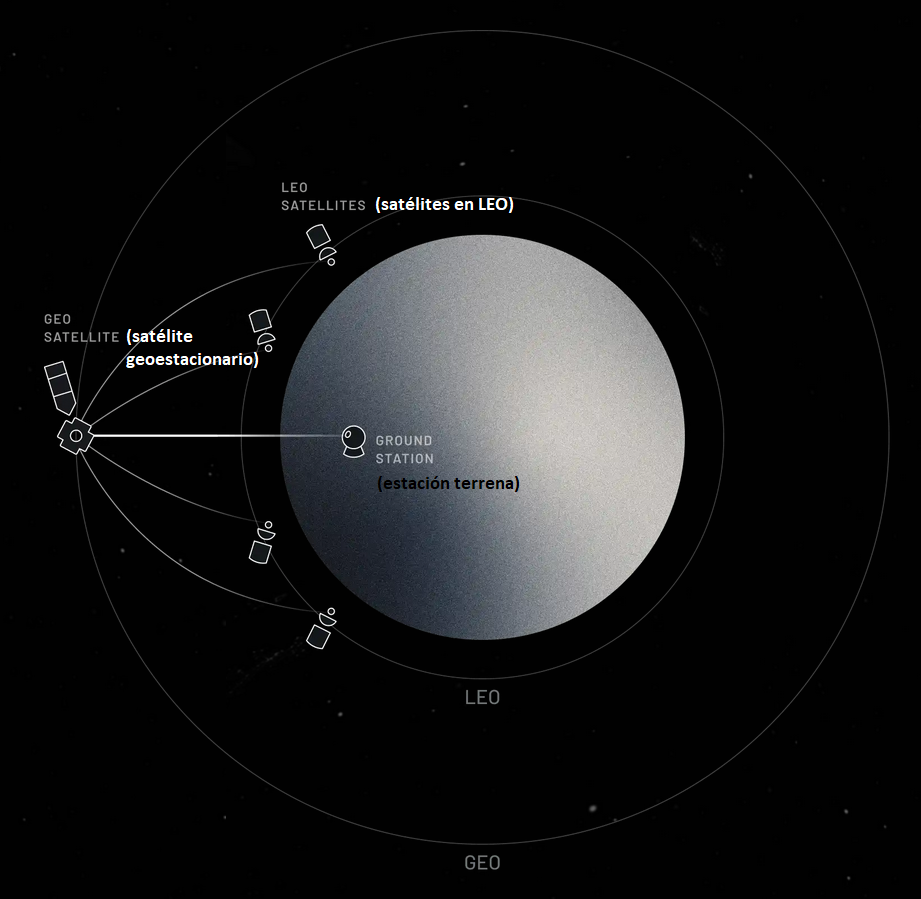
\includegraphics[width=0.8\textwidth]{./Figures/propuesta_skyloom.png}
\caption{Propuesta de la empresa Skyloom Global\protect\footnotemark.}
\label{fig:propSky}
\end{figure}

\footnotetext{Imagen tomada de \url{https://www.skyloom.co/}}

El enlace óptico, que permite la transmisión y recepción de datos a una velocidad de 1 Gbps (1 \textit{Gigabit} por segundo) entre satélites, se establece mediante una terminal de comunicaciones óptica, que es el principal producto actualmente en desarrollo por la empresa. Estas terminales cuentan con un láser que trabaja sobre una longitud de onda de 1550 nm (banda C del espectro). Dicho láser es el encargado de transmitir la información propiamente dicha mediante pulsos de luz (no visible).

En líneas generales, los láseres de esta longitud de onda que se encuentran en el mercado no cuentan con la potencia óptica necesaria para que sean detectados por el receptor. Esto se debe principalmente a que la distancia de espacio libre estimada entre dos satélites en LEO es de unos 4000 km \citep{WEBSITE_SKY}.

Para solucionar el problema antes mencionado, se introduce a la salida del láser un amplificador dopado con erbio o EDFA (del inglés, \textit{Erbuim Doped Fiber Amplifier}) \citep{WEBSITE:EDFA2}. La función de este dispositivo es aumentar la potencia del láser varias veces, de forma que se alcance un nivel adecuado para la transmisión.

El modelo de amplificador utilizado por la empresa cuenta con un conector que provee una interfaz electrónica para poder controlar su funcionamiento. Esta interfaz cuenta con distintas señales y buses de comunicación que se explican con mayor detalle en la sección \ref{sec:intAmp}.

Este amplificador formará parte de la terminal de comunicaciones y estará sometido a intensivas pruebas de funcionamiento y rendimiento durante la etapa de investigación y desarrollo. Para esto, es indispensable contar con una herramienta que permita a los ingenieros a cargo utilizar el amplificador de forma aislada, es decir, sin depender del hardware del producto final.

En la figura \ref{fig:bloquesProy} se puede ver un esquema de uso del dispositivo y sus conexiones con el hardware externo.

\begin{figure}[H]
\centering
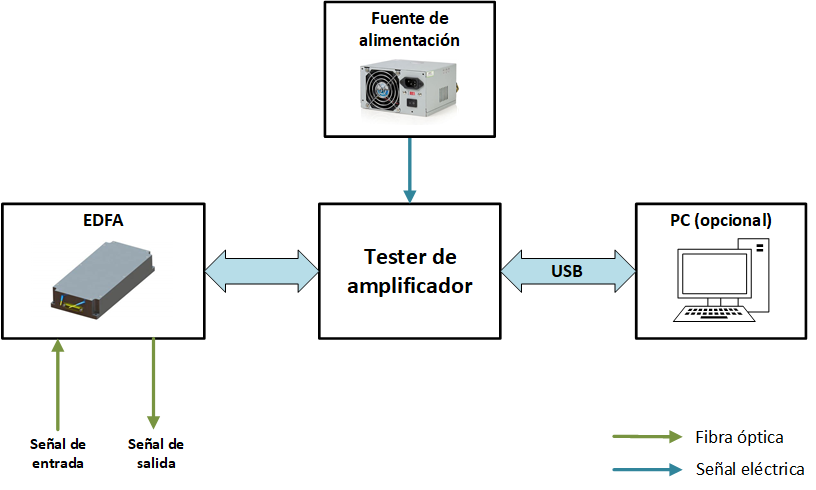
\includegraphics[width=0.85\textwidth]{./Figures/bloquesProy.png}
\caption{Esquema de uso y conexionado del sistema.}
\label{fig:bloquesProy}
\end{figure}

El dispositivo cuenta con tres conexiones externas: la interfaz con el amplificador, la conexión a la fuente de alimentación y un puerto USB.

La interfaz con el EDFA permite controlarlo y consultar diversos parámetros de funcionamiento a través de las señales presentes en el conector. La fuente de alimentación se encarga de energizar el tester y el EDFA. Y por último, la conexión USB permite controlar el amplificador del mismo modo que en el tester, por lo que el uso de la PC es opcional. Para poder hacer esto, sobre esta debe correr un software que permita establecer una comunicación.

%----------------------------------------------------------------------------------------

\section{Estado del arte}

Si bien hoy en día los EDFA son ampliamente utilizados en varias aplicaciones de optoelectrónica, en la actualidad no existe un estándar para la interfaz eléctrica que poseen estos amplificadores. Esto lleva a que cada fabricante defina una propia para sus productos y que el usuario tenga que adaptar su hardware para poder usarlos.

Para el caso en que se necesite contar con un tester o una placa de depuración para hacer uso o pruebas sobre el dispositivo, el usuario debe adquirir una del mismo fabricante del amplificador por esta misma razón. Actualmente, la empresa hace uso de una de estas placas, la cual se puede ver en la figura \ref{fig:placaDebug}.

\begin{figure}[H]
\centering
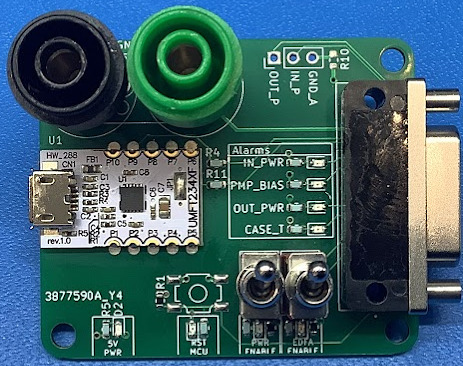
\includegraphics[width=0.60\textwidth]{./Figures/placaDebug.jpg}
\caption{Placa de depuración.}
\label{fig:placaDebug}
\end{figure}

Esta placa, denominada EDFA IFC (Interface Card), cuenta con la electrónica necesaria para proveer al usuario algunas funcionalidades básicas que le permiten hacer uso del amplificador. Contiene una interfaz USB-UART para usarse junto con una computadora, LEDs para las señales de alarmas y conectores para la alimentación del EDFA.

\section{Motivación}

La empresa ya lleva algún tiempo haciendo uso de la placa mecionada en la sección anterior y recientemente ha tomado la decisión de dejar de usarla y diseñar una propia debido a los motivos que se listan a continuación:

\begin{itemize}
\item No permite el uso de todas las señales presentes en la interfaz del amplificador.
\item Tiene una tasa de fallas muy alta, en particular la interfaz UART.
\item Su costo es muy elevado en relación a sus prestaciones.
\item El tiempo de entrega del producto es de varias semanas.
\item No posee las protecciones eléctricas necesarias para proteger el amplificador.
\end{itemize}

Las desventajas aquí expuestas son los principales motivos que dieron origen a la necesidad de contar con el sistema propuesto en este trabajo. Esto le permite a la empresa no depender del fabricante para la entrega de estos testers y por lo tanto reducir costos y tiempos.

Por otro lado, el tester desarrollado en este trabajo no solo posee las mismas funcionalidades que el ofrecido por el fabricante sino que también incorpora otras características adicionales que lo hacen más fácil de usar, menos propenso a fallas y más seguro.

%----------------------------------------------------------------------------------------

\section{Objetivos y alcance}

El objetivo principal de este trabajo fue el desarrollo de un dispositivo capaz de controlar y realizar mediciones sobre un amplificador de fibra óptica. Las tareas contempladas fueron:

\begin{itemize}
\item Diseño y construcción de un prototipo funcional del dispositivo.
\item Diseño e implementación del firmware del dispositivo.
\item Diseño de los bancos de prueba y ensayos.
\item Simulación del funcionamiento del hardware mediante software.
\item Documentación de diseño y manual de uso.
\end{itemize}

Los puntos del desarrollo que no se contemplaron en el trabajo fueron:

\begin{itemize}
\item Diseño y construcción de la versión final del dispositivo.
\item Especificación de las pruebas a ejecutar sobre el amplificador óptico utilizando el dispositivo.
\item Fabricación del PCB del dispositivo.
\item Procesamiento e interpretación de los valores de los parámetros del EDFA.
\item Diseño y construcción de la fuente de alimentación externa.
\item Diseño e implementación del software a ejecutarse en la PC.
\end{itemize}


%----------------------------------------------------------------------------------------

\chapter{Introducción específica} % Main chapter title

\label{Chapter2}

%----------------------------------------------------------------------------------------
%	Chapter 2
%----------------------------------------------------------------------------------------

Este capítulo lista los requerimientos y en base a ellos presenta y describe los componentes internos del sistema desarrollado, junto con las tecnologías y recursos de software utilizados para su implementación. Asimismo, se realiza una descripción simplificada del funcionamiento de un EDFA.

\section{Requerimientos}
\label{sec:reqs}

Los requerimientos fueron determinados en conjunto con la empresa en base a las funcionalidades y prestaciones con las que debe contar el sistema. Como la lista es muy extensa, se listan a continuación solamente algunos de los principales:

\renewcommand{\labelenumii}{\arabic{enumi}.\arabic{enumii}}

\begin{enumerate}

\item Encendido y apagado del EDFA
	\begin{enumerate}
	\item El software debe apagar la salida óptica del dispositivo 			EDFA bajo prueba cuando se detecte la activación de alguna de las 		alarmas.
	\item Mediante la función táctil de la pantalla LCD el usuario 			debe poder prender y apagar la alimentación del dispositivo EDFA 		bajo prueba y su salida óptica.
	\item El software debe cortar la alimentación del dispositivo EDFA 	bajo prueba cuando se detecte que la corriente supera el valor 			previamente definido.
	\item El software debe medir y mostrar en pantalla los valores de 		tensión de alimentación y consumo de corriente del dispositivo 			EDFA bajo prueba mediante las señales analógicas de entrada 			provenientes de los respectivos monitores, con una precisión no 		menor al 10\% (máximo desvío con respecto al valor real). Este 			valor debe ser de una cifra significativa para la parte entera y 		dos para la decimal.
	\end{enumerate}

\item Pantalla LCD
	\begin{enumerate}
	\item El software debe actualizar la imagen de la pantalla cada 		medio segundo (2 cuadros por segundo).
	\item La pantalla deberá indicar el estado de la salida óptica del 	dispositivo EDFA bajo prueba y el del relé de alimentación.
	\item Mediante la función táctil de la pantalla LCD el usuario 			debe poder cambiar el valor para el cual se detecta una 				sobrecorriente. El rango válido para este valor debe ser de 0 A a 		3 A, siendo la parte decimal de dos cifras significativas.
	\end{enumerate}
	
\item Entradas y salidas del EDFA
	\begin{enumerate}
	\item El software deberá mostrar en la pantalla los estados de todas las señales digitales de entrada y salida del dispositivo EDFA bajo prueba.
	\end{enumerate}

\item Requisitos de rendimiento
	\begin{enumerate}
	\item \label{item:req1} La apertura del relé de alimentación del dispositivo EDFA 		bajo prueba deberá efectuarse en un tiempo menor a 50 ms luego de 		detectarse una sobrecorriente o una caída de la tensión de 				alimentación.
	\item \label{item:req2} El apagado de la salida óptica del dispositivo EDFA bajo 			prueba deberá efectuarse en un tiempo menor a 100 ms luego de 			detectarse la activación de una alarma.
	\end{enumerate}
	
\end{enumerate}

La lista completa de requerimientos se puede ver en \citep{DOC_REQ}.

\section{Funcionamiento de un amplificador óptico}
\label{sec:funcAmp}

Los amplificadores de fibra dopados con erbio son los amplificadores ópticos más importantes en el contexto de comunicaciones ópticas de larga distancia. Son utilizados en la banda L y C del espectro (aproximadamente entre 1530 nm y 1625 nm \citep{WEBSITE:BANDAS}), región en la que las pérdidas en la fibra óptica son menores. Esto se puede ver en la figura \ref{fig:espectro}, que muestra las pérdidas en función de la longitud de onda de la luz utilizada.

\begin{figure}[H]
\centering
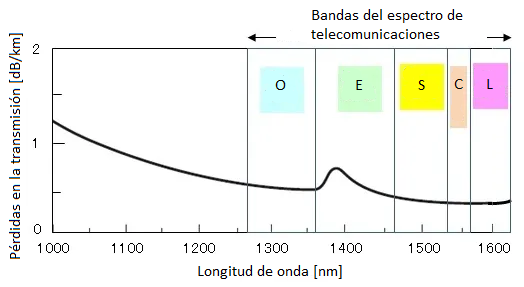
\includegraphics[width=0.85\textwidth]{./Figures/espectro.png}
\caption{Pérdidas en la fibra\protect\footnotemark.}
\label{fig:espectro}
\end{figure}

\footnotetext{Imagen tomada de \citep{WEBSITE:BANDAS}}

Inventado en 1987 \citep{WEBSITE:EDFA1}, el EDFA es generalmente usado para compensar las pérdidas mencionadas en una línea de transmisión óptica. Este puede ser colocado en tres partes: 

\begin{itemize}
\item Inmediatamente después del transmisor, para aumentar la potencia inyectada en la línea.
\item En el medio del camino óptico, para compensar las pérdidas por la distancia recorrida.
\item Antes del receptor, para favorecer la detección de la señal.
\end{itemize}

La figura \ref{fig:EDFAinterno} muestra la configuración interna más común de un EDFA. Su componente principal es la fibra dopada con erbio (EDF por sus siglas en inglés), que generalmente es monomodo \citep{WEBSITE:FIBRA}. 

La luz ingresa al amplificador mediante el puerto de entrada y luego mediante un divisor se redirige un porcentaje de la señal (generalmente entre un 1\% y 2\% \citep{WEBSITE:EDFA2}) a un detector para realizar una medición de la potencia óptica. Luego, pasa por un aislador óptico que permite la transmisión de luz en un solo sentido y así evita una realimentación debida a reflexiones en etapas posteriores.

La bomba de 980 nm es un diodo láser que genera una señal lumínica en esa longitud de onda. Esta luego se mezcla con la señal de luz entrante (a la salida del aislador) y atraviesan la fibra dopada con erbio. En esta instancia es donde se genera la amplificación de la señal propiamente dicha, mediante un efecto denominado emisión estimulada \citep{WEBSITE:EDFA2}\citep{WEBSITE:EMISSION}.

\begin{figure}[H]
\centering
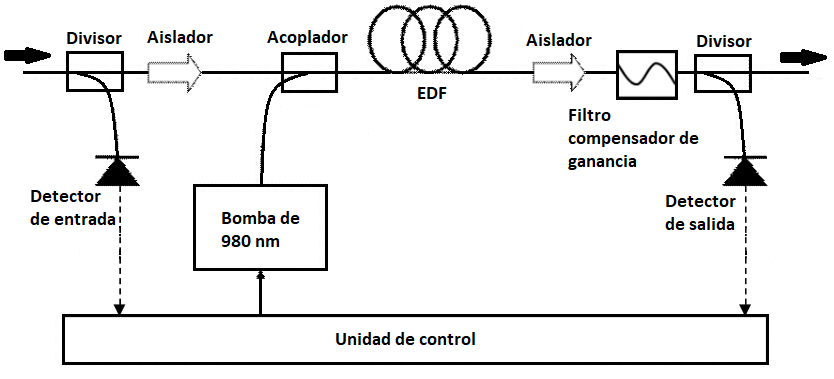
\includegraphics[width=0.85\textwidth]{./Figures/EDFAinterno.png}
\caption{Configuración interna de un EDFA\protect\footnotemark.}
\label{fig:EDFAinterno}
\end{figure}

\footnotetext{Imagen tomada de \citep{WEBSITE:EDFA2}}

Una vez amplificada, la señal pasa nuevamente por otro aislador que se encarga principalmente de filtrar la luz de 980 nm, evitando que se introduzca en el camino óptico. Luego, la señal pasa por un filtro aplanador de ganancia (GFF por sus siglas en inglés) cuyo objetivo es hacer constante la ganancia del amplificador en todo el ancho de banda de trabajo \citep{WEBSITE:EDFA3} (bandas C y L del espectro). Finalmente, antes de que la luz salga del amplificador, se realiza nuevamente una medición de la potencia óptica al igual que en la entrada.

Tanto la bomba de 980 nm como ambos detectores de potencia se encuentran conectados a una unidad de control. Esta generalmente cuenta con un microcontrolador o chip dedicado que se encarga de regular la potencia que entrega la bomba en base a los valores medidos por los detectores, creando un lazo de control automático de ganancia \citep{WEBSITE:EDFA2}\citep{WEBSITE:EDFA1}.

\section{Interfaz del amplificador óptico}
\label{sec:intAmp}

Como se mencionó en la sección \ref{sec:contexto}, para poder controlarlo, el EDFA cuenta con un conector de 25 pines tipo Micro-D \citep{WEBSITE:MICROD_DS}. Este conector contiene varios grupos de señales con distintas funciones. La tabla \ref{tab:señalesConector} lista cada una de las señales de la interfaz, junto con los detalles de su dirección, tipo y función.

\begin{table}[H]
	\centering
	\caption{Señales de la interfaz del EDFA.}
	\begin{tabular}{l c p{1.5cm} p{5cm}}
		\toprule
		\textbf{Nombre de la señal}	& \textbf{Dirección}	& \textbf{Tipo} & \textbf{Función} \\
		\midrule
		5 V 					& Entrada	& Potencia			& Entrada de alimentación del EDFA. \\		
		PGND				& Salida	& Potencia  		& Retorno de alimentación (potencia). \\
		GND					& Salida	& Tierra digital  	& Retorno de alimentación (digital). \\
		IN\_POW				& Salida	& Analógica 		& Indica el nivel de potencia óptica de entrada. \\
		OUT\_POW			& Salida	& Analógica 		& Indica el nivel de potencia óptica de salida. \\
		CASE\_TEMP\_ALARM	& Salida	& Digital 			& Alarma de temperatura de la carcasa del EDFA. \\
		PUMP\_BIAS\_ALARM	& Salida	& Digital 			& Alarma de la bomba de polarización. \\
		OUT\_POW\_ALARM		& Salida	& Digital 			& Alarma de nivel de potencia de salida. \\
		IN\_POW\_ALARM		& Salida	& Digital 			& Alarma de nivel de potencia de entrada. \\
		EN/DIS				& Entrada	& Digital 			& Habilitación del amplificador. \\
		RESET\_uC			& Entrada	& Digital 			& Reset del microcontrolador del EDFA. \\
		OUT\_POW\_MUTE		& Entrada	& Digital 			& Habilitación de la salida óptica. \\
		UART\_TX			& Salida	& Digital 			& Transmisor del UART interno del EDFA. \\
		UART\_RX			& Entrada	& Digital 			& Receptor del UART interno del EDFA. \\
		\bottomrule
		\hline
	\end{tabular}
	\label{tab:señalesConector}
\end{table}

A continuación, se provee una breve explicación de cada grupo de señales:
\begin{itemize}
\item Alimentación: tiene separada la tierra en digital, para la lógica y la comunicación, y la de potencia para la amplificación de la señal óptica.
\item Señales analógicas: indican el nivel de potencia óptica de entrada y salida del EDFA.
\item Alarmas: mediante un estado en alto indican si ocurrió alguno de los eventos que requieren la atención del usuario.
\item Señales de control: controlan el funcionamiento de ciertos componentes del amplificador.
\item Comunicación UART: permite el envío de comandos al EDFA y la consulta de valores de parámetros internos como temperaturas, potencias, ganancias, etc.
\end{itemize}

\section{Componentes del sistema}

Los componentes de hardware que conforman el sistema descrito en la sección \ref{sec:contexto} fueron seleccionados con el objetivo de cumplir con los requisitos, optimizando al mismo tiempo la cantidad de elementos utilizados. Así se logra mantener al sistema simple, con poca probabilidad de fallas, fácil de usar y probar. A continuación se presentan los principales componentes y sus características.

\subsection{Microcontrolador}

El modelo de microcontrolador utilizado es el STM32F429 \citep{STM32F429}, del fabricante ST y con arquitectura de procesador Arm Cortex-M. La principal razón por la que se decidió utilizar este modelo es porque es el que se encuentra integrado en la placa de desarrollo NUCLEO-144, utilizada durante la cursada de la especialización.

La placa de desarrollo NUCLEO-144 es ideal para ejecutar un RTOS debido a su alta velocidad de reloj, gran capacidad de memoria flash y variedad de periféricos, además de contar con la ventaja de tener integrada la interfaz de programación y depuración ST-LINK/V2 \citep{NUCLEO144}.

\subsection{Monitor de corriente}

El circuito integrado seleccionado para medir la corriente de alimentación del amplificador mientras está en funcionamiento es el INA301A3 \citep{INA301}.

Este chip provee en uno de sus pines una tensión analógica proporcional a la corriente que se está midiendo. Asimismo, cuenta con una salida digital que se activa cuando la corriente medida alcanza cierto nivel establecido mediante un resistor (pin ALERT) \citep{INA301}.

\subsection{Pantalla táctil LCD}
\label{sec:pantLCD}

El modelo del módulo de la pantalla LCD utilizada en el trabajo es MSP2807 \citep{MSP2807}, que es una solución integrada, es decir, cuenta con toda la electrónica necesaria para poder hacer uso de la pantalla en su totalidad. Para esto cuenta con dos circuitos integrados: el controlador del display de la pantalla (lo que permite dibujar en ella) y el controlador de la función táctil (lo que permite detectar cuando se la toca). En la figura \ref{fig:pantLCD} se puede ver una imagen de la pantalla.

\begin{figure}[H]
\centering
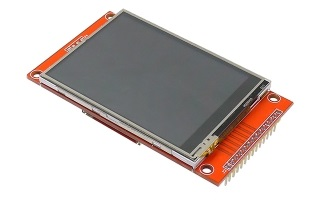
\includegraphics[width=0.7\textwidth]{./Figures/pant_LCD.png}
\caption{Pantalla LCD táctil MSP2807\protect\footnotemark.}
\label{fig:pantLCD}
\end{figure}

\footnotetext{Imagen tomada de \citep{MSP2807}}

El controlador del display utiliza una interfaz SPI para la recepción de datos y cuenta con una señal DC/RS para distinguir entre datos y registros internos. El controlador táctil también opera mediante SPI y dispone de una señal de interrupción T\_IRQ que indica cuando se ha producido una interacción en la pantalla \citep{MSP2807}.

\section{Recursos de software}

Para el firmware del microcontrolador se usaron distintas herramientas que permitieron el desarrollo de una estructura de software jerárquica, simple y eficaz.

\subsection{Sistema operativo de tiempo real FreeRTOS}

FreeRTOS es un sistema operativo de tiempo real (RTOS) diseñado para microcontroladores y microprocesadores pequeños. Se caracteriza por ser liviano, confiable y fácil de usar. Ofrece recursos como tareas, semáforos, \textit{mutexes}, colas y gestores de memoria dinámica \citep{WEBSITE:1}, lo que simplifica la creación y gestión de aplicaciones sobre el sistema operativo.

FreeRTOS se sitúa en una capa intermedia del firmware, por encima de los drivers del fabricante y debajo de la aplicación de usuario, brindando una capa de abstracción que automatiza la gestión de los recursos de hardware. Su principal ventaja es la capacidad de ejecutar múltiples tareas o procesos de manera simultánea. Esto permite estructurar aplicaciones en tareas independientes y sincronizadas \citep{WEBSITE:FREERTOS}.

\subsection{Capa de abstracción de hardware (HAL)}

Una \textit{hardware abstraction layer} o HAL es un conjunto de rutinas de software que brinda acceso a recursos de hardware a programas de aplicación. Se ubica inmediatamente por arriba del hardware y por debajo del sistema operativo que se ejecuta.

La principal ventaja de esta capa es que oculta la arquitectura del hardware del \textit{kernel} del sistema operativo. Así, el código del \textit{kernel} no tiene que ser cambiado o reescrito para que pueda correr sobre sistemas con distinto hardware y las aplicaciones de software se vuelven independientes de la plataforma (portabilidad) \citep{WEBSITE:HAL}.

La HAL de la serie de microcontroladores STM32 se denomina STM32Cube y tiene como objetivo asegurar la máxima portabilidad entre dispositivos de la misma familia y proveer APIs (\textit{Application Programming Interface}) multi-instancia para todos los periféricos (UART, SPI, temporizadores, ADC, etc.). Estas APIs están listas para usar y facilitan la implementación de la aplicación de usuario. Por ejemplo, los periféricos de comunicación cuentan con APIs para inicializarlos y configurarlos, gestionar la transferencia de datos en modo \textit{polling}, manejar las interrupciones, el DMA (\textit{Direct Memory Access}) y los errores de comunicación \citep{WEBSITE:STM32CUBE}.

\section{Periféricos utilizados}

A excepción del monitor de corriente, el resto de los periféricos utilizados ya se encuentran integrados en el chip del microcontrolador, por lo que no hubo necesidad de agregar ningún hardware adicional.

\subsection{Conversor analógico-digital (ADC)}

Un conversor analógico-digital o ADC es un dispositivo que convierte una señal eléctrica analógica proveniente, por ejemplo, de un sensor a una señal digital. De esta forma su valor puede ser almacenado en un sistema digital, por lo que estará representada por un número binario \citep{WEBSITE:2}.

\subsection{Universal Asynchronous Receiver Transmitter (UART)}

Un UART es un dispositivo utilizado para establecer una comunicación serie asíncrona, con formato de datos y velocidad de transmisión configurables. Consta solo de dos señales que conectan dos dispositivos de forma bidireccional: una para la transmisión y otra para la recepción, comúnmente llamadas TX y RX respectivamente \citep{WEBSITE:3}.

\subsection{Serial Peripheral Interface (SPI)}

SPI es una especificación de interfaz de comunicación serie sincrónica para distancias cortas. Es comúnmente utilizada para enviar datos entre un sistema embebido y pequeños periféricos como sensores y memorias SD.

Los dispositivos SPI se comunican en modo \textit{full duplex} (ambos sentidos simultáneos) y cuentan con una señal de clock, dato entrante, dato saliente y de selección de esclavo, que conecta o desconecta la operación del dispositivo con el que uno desea comunicarse. De esta forma, este estándar permite multiplexar las líneas de clock y soportar arquitecturas multi-esclavo \citep{WEBSITE:SPI}.


\chapter{Diseño e implementación} % Main chapter title

\label{Chapter3} % Change X to a consecutive number; for referencing this chapter elsewhere, use \ref{ChapterX}

\definecolor{mygreen}{rgb}{0,0.6,0}
\definecolor{mygray}{rgb}{0.5,0.5,0.5}
\definecolor{mymauve}{rgb}{0.58,0,0.82}

%%%%%%%%%%%%%%%%%%%%%%%%%%%%%%%%%%%%%%%%%%%%%%%%%%%%%%%%%%%%%%%%%%%%%%%%%%%%%
% parámetros para configurar el formato del código en los entornos lstlisting
%%%%%%%%%%%%%%%%%%%%%%%%%%%%%%%%%%%%%%%%%%%%%%%%%%%%%%%%%%%%%%%%%%%%%%%%%%%%%
\lstset{ %
  backgroundcolor=\color{white},   % choose the background color; you must add \usepackage{color} or \usepackage{xcolor}
  basicstyle=\footnotesize,        % the size of the fonts that are used for the code
  breakatwhitespace=false,         % sets if automatic breaks should only happen at whitespace
  breaklines=true,                 % sets automatic line breaking
  captionpos=b,                    % sets the caption-position to bottom
  commentstyle=\color{mygreen},    % comment style
  deletekeywords={...},            % if you want to delete keywords from the given language
  %escapeinside={\%*}{*)},          % if you want to add LaTeX within your code
  %extendedchars=true,              % lets you use non-ASCII characters; for 8-bits encodings only, does not work with UTF-8
  %frame=single,	                % adds a frame around the code
  keepspaces=true,                 % keeps spaces in text, useful for keeping indentation of code (possibly needs columns=flexible)
  keywordstyle=\color{blue},       % keyword style
  language=[ANSI]C,                % the language of the code
  %otherkeywords={*,...},           % if you want to add more keywords to the set
  numbers=left,                    % where to put the line-numbers; possible values are (none, left, right)
  numbersep=5pt,                   % how far the line-numbers are from the code
  numberstyle=\tiny\color{mygray}, % the style that is used for the line-numbers
  rulecolor=\color{black},         % if not set, the frame-color may be changed on line-breaks within not-black text (e.g. comments (green here))
  showspaces=false,                % show spaces everywhere adding particular underscores; it overrides 'showstringspaces'
  showstringspaces=false,          % underline spaces within strings only
  showtabs=false,                  % show tabs within strings adding particular underscores
  stepnumber=1,                    % the step between two line-numbers. If it's 1, each line will be numbered
  stringstyle=\color{mymauve},     % string literal style
  tabsize=2,	                   % sets default tabsize to 2 spaces
  title=\lstname,                  % show the filename of files included with \lstinputlisting; also try caption instead of title
  morecomment=[s]{/*}{*/}
}


%----------------------------------------------------------------------------------------
%	Chapter 3
%----------------------------------------------------------------------------------------

En este capítulo se realiza una explicación detallada del diseño del hardware, cómo se utilizó cada componente principal y su conexión con el microcontrolador. Asimismo, se especifica la estructura general del firmware en el marco de FreeRTOS y las principales rutinas de bajo nivel.


\section{Arquitectura de hardware}

La arquitectura general de la placa fue diseñada para tener como unidad de procesamiento principal al microcontrolador STM32 de la placa NUCLEO-144 y a la pantalla LCD como periférico principal de salida de datos.

La figura \ref{fig:estrucInt} muestra un diagrama completo de todo el hardware de la placa fabricada, sus entradas, salidas y el conexionado entre sus distintas partes. También incluye los periféricos utilizados en el microcontrolador y la cantidad de líneas de cada conexión.

\begin{figure}[H]
\centering
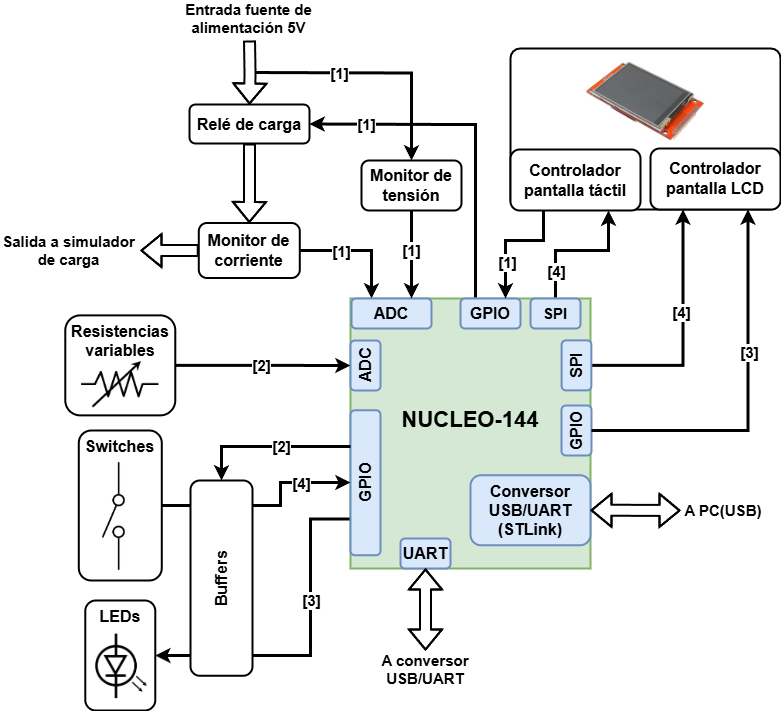
\includegraphics[width=0.84\textwidth]{./Figures/diagDisp.png}
\caption{Diagrama completo del hardware implementado.}
\label{fig:estrucInt}
\end{figure}

Todos los bloques externos a la placa NUCLEO que se ven en el diagrama, a excepción de la pantalla LCD, fueron diseñados con componentes electrónicos básicos, es decir, sin usar módulos funcionales compactos.

Los bloques internos de la placa NUCLEO que se ven en el diagrama, a excepción del conversor USB-UART, son periféricos que se encuentran embebidos en el mismo chip del microcontrolador. El conversor USB-UART, denominado STLink, se encuentra fuera de este y esta compuesto por varios componentes electrónicos.

En el apéndice \ref{AppendixA} se encuentra el diseño esquemático completo de la placa.

\subsection{Medición de corriente del amplificador}

El principio de funcionamiento del monitor de corriente se basa en un resistor \textit{shunt}, el cual se coloca sobre la alimentación, en serie con la línea a la que se desea conocer el consumo de corriente. Para que este resistor no disipe mucha potencia y disminuya la tensión de la línea, su valor de resistencia es de 10 \si{m\ohm}. Mientras menos comparable sea su valor al de la carga más despreciables serán los efectos negativos que introducirá.

Sobre este resistor cae una tensión proporcional a la corriente consumida por el EDFA. Como el valor máximo de corriente consumida por el amplificador se encuentra cerca de los 2,5 A, sobre el resistor caen como máximo 25 mV, lo que frente a los 5 V de la alimentación no representa un valor significativo. Luego de sensarla, el chip amplifica 100 veces esta tensión diferencial y la conecta a uno de sus pines de salida.

Al ser este un valor analógico, para poder ser interpretado se lo debe convertir a digital. Para esto se usa el ADC incorporado en el microcontrolador, conectando a uno de sus pines la señal de salida del monitor de corriente. La tensión máxima que puede alcanzar la señal es de aproximadamente 2,5 V, lo que se encuentra por debajo de la tensión de referencia del ADC. Un esquema de esta conexión se puede ver en la figura \ref{fig:funcMonitor}.

\begin{figure}[H]
\centering
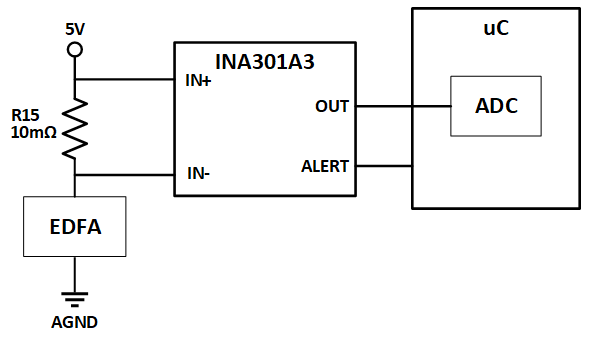
\includegraphics[width=0.75\textwidth]{./Figures/func_monitor.png}
\caption{Esquema del monitor de corriente.}
\label{fig:funcMonitor}
\end{figure}

Por otro lado, el INA301A3 cuenta con un pin de salida denominado ALERT que se activa cuando la corriente medida alcanza cierto valor, lo que funciona a modo de alarma. Este nivel se determina conectando un resistor de cierto valor en el pin LIMIT.

\subsection{Relé de alimentación}

La línea de 5 V de alimentación del EDFA es controlada mediante la activación de un relé (código APAN3103) \citep{WEBSITE:RELE_DS}, lo que significa que la conexión y desconexión es mecánica. Esto se decidió implementarlo así debido a los lineamientos de protecciones necesarios para el hardware de vuelo.

Como el relé necesita de aproximadamente 36,7 mA para activarse, no se puede conectar directamente a un pin de salida del microcontrolador ya que este no puede suministrar la corriente necesaria. Por esta razón la activación se realiza mediante un transistor (código MMBT2222) \citep{WEBSITE:TRANS_DS}, funcionando como una llave (en modo saturación o corte). De esta forma, la corriente para la activación de la bobina del relé la provee directamente la fuente de alimentación de 3,3 V.

\subsection{Medición de tensión del amplificador}

Hacer una medición de la tensión de la línea es mucho más sencillo que hacer una medición de la corriente, ya que esta se puede conectar directamente a un ADC si previamente se la atenúa o amplifica (dependiendo del caso).

En este caso, como la tensión de alimentación del EDFA es 5 V y la tensión de referencia del ADC del microcontrolador es 3,3 V, se la debe atenuar de forma que esta se encuentre dentro del fondo de escala del ADC.

Considerando que se desea medir una sobretensión de por lo menos 1 V en la alimentación, se opta por atenuar la tensión del EDFA a la mitad, resultando en un fondo de escala de 6,6 V.

Esta técnica permite medir tensiones mayores a la de referencia del ADC pero trae como desventaja que se pierde precisión debido al ruido y la tolerancia de los resistores.

En la figura \ref{fig:monTension} se puede ver el circuito implementado.

\begin{figure}[H]
\centering
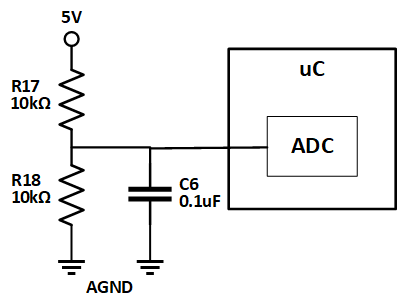
\includegraphics[width=0.5\textwidth]{./Figures/mon_tension.png}
\caption{Circuito del monitor de corriente.}
\label{fig:monTension}
\end{figure}

El capacitor C6 forma un filtro RC \citep{WEBSITE:RC_CIRCUIT} para eliminar el ruido de alta frecuencia que pueda tener la línea.

\subsection{Conexión a pantalla LCD}
\label{sec:conLCD}

Como se puede ver en la figura \ref{fig:estrucInt}, la pantalla LCD tiene dos controladores con SPI: uno para el control de la pantalla y otro para el control de la función táctil. Si bien ambas interfaces se podrían haber conectado al mismo periférico SPI del microcontrolador en modo multi-esclavo, se decidió usar uno para cada uno de forma individual. La principal razón de esto es porque facilita la implementación del firmware ya que permite usar ambos controladores de forma independiente y a distintas velocidades sin necesidad de reconfiguración.

El controlador de la función táctil tiene, además de las señales del bus SPI, una señal denominada IRQ que se activa cuando se detecta que la pantalla está siendo tocada. Esta señal sirve para ser usada como interrupción en el programa del microcontrolador.

Por otro lado, el controlador del display también tiene señales con funciones especiales. Estas son:

\begin{itemize}
\item RESET: resetea el chip del controlador y, por lo tanto, toda la configuración del display y la información de cada píxel.
\item DC/RS: indica al controlador si la información que se está enviando por el SPI es un dato o un registro, dependiendo del nivel de la señal.
\item LED: permite controlar la intensidad de luz de la pantalla (denominada \textit{backlight}).
\end{itemize}

\subsection{Entradas y salidas digitales}

En la tabla \ref{tab:señalesConector} se detallan las señales de entrada y salida digitales del puerto del EDFA. Las salidas son señales de alarmas y las de entrada, de control.

Estas señales se podrían conectar directamente a pines digitales del microcontrolador ya que son de tipo TTL 3,3 V, pero se decidió poner antes de este un \textit{buffer} de tres estados (código SN74LVC2244A) \citep{WEBSITE:BUFFERS_DS}. Los objetivos de esta decisión son tres:

\begin{itemize}
\item Generar niveles de tensión mejor definidos. Esto filtra ruido y rebote en las señales y facilita la detección en ambos extremos (EDFA y microcontrolador).
\item Proveer a la electrónica interna del EDFA de protección contra descargas electrostáticas (ESD).
\item Suministrar la corriente necesaria a las señales de entrada del amplificador y así evitar que esta deba ser proporcionada por el microcontrolador.
\end{itemize}

Para poder simular la activación de las alarmas en la placa se colocaron pulsadores con testigo lumínico (código TL1265YQSCLR) \citep{WEBSITE:PULSADOR_DS} en el extremo donde estaría el EDFA, con el propósito de activarlos manualmente durante el testeo del firmware.

Para las señales de control se utilizaron LEDs que indican el estado de activación de estas (código AA3528LVBS/D) \citep{WEBSITE:LEDS_DS}.

\subsection{Indicadores de potencia óptica}

Las señales IN\_POW y OUT\_POW son analógicas y pueden tomar cualquier valor en el rango de 0 V a 3,3 V. Este valor es proporcional a la potencia óptica medida por los detectores de entrada y salida del amplificador, el cual corresponde al rango de -10 dBm a 10 dBm para el de entrada y 5 dBm a 37 dBm para el de salida.

Para poder simular estas señales se utilizaron dos resistores variables (código PTV09A-4020U-B103) \citep{WEBSITE:POTENC_DS} que permiten variar de forma manual el valor de tensión entre 0 V y 3,3 V.

\subsection{Interfaz UART}

Como se puede ver en la figura \ref{fig:estrucInt}, el dispositivo debe contar con dos interfaces UART: una para la comunicación entre el tester y el EDFA y otra para la comunicación entre el tester y la PC. Para esto se requiere hacer uso de dos de los controladores UART internos que posee el microcontrolador.

\section{Arquitectura de firmware}

Como se mencionó anteriormente, la arquitectura del firmware del trabajo tiene como base la utilización de FreeRTOS y los recursos que ofrece. Esto permite la implementación de un diseño eficaz y sencillo mediante la división en dos partes bien definidas: la parte de procesamiento de datos y control (o backend) y la parte gráfica que interactúa con el usuario (o frontend). Para implementar cada una de ellas se utilizó una tarea o proceso, recurso provisto por el sistema operativo. Como la velocidad de reloj del microcontrolador es alta, se puede asumir que estas se ejecutan de forma independiente y simultánea. Por otro lado, estas comparten ciertas variables cuyo acceso debe ser controlado para que no existan colisiones de lectura o escritura. Este acceso es gestionado por un semáforo.

El proceso del backend tiene como tarea principal ejecutar una máquina de estados y se encarga de controlar el estado general del dispositivo en todo momento. Esto significa que lee los datos de entrada, los procesa y en base a ellos toma decisiones que terminan por afectar las señales de salida y en última instancia a la tarea del display. A demás, ejecuta una consola de control que le permite al usuario interactuar con el tester e indirectamente con el EDFA. 

Por otro lado, el proceso del frontend esta asociado al display LCD y tiene como objetivo principal la interacción directa con el usuario. Para ello, debe leer la información de salida del backend, presentarla en la pantalla y, a su vez, detectar cuándo y dónde el usuario presiona sobre ella y enviar estos datos al backend mediante recursos compartidos. 

En la figura \ref{fig:arqFW} se puede ver un diagrama de cómo se relacionan ambas tareas entre sí y con el hardware.

\begin{figure}[H]
\centering
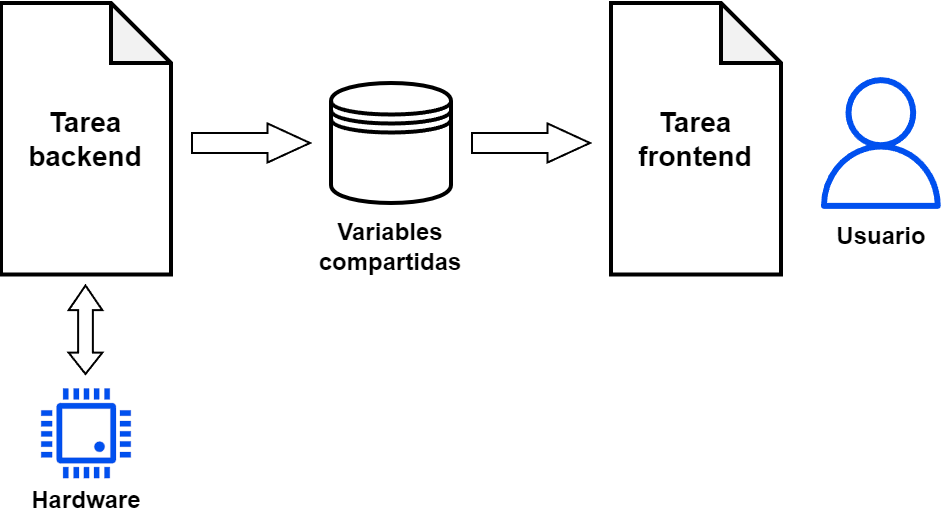
\includegraphics[width=0.85\textwidth]{./Figures/arqFW.png}
\caption{Arquitectura de firmware.}
\label{fig:arqFW}
\end{figure}

\subsection{Tarea del backend}

El proceso del backend ejecuta las funciones más importantes del programa de forma continua. Estas son la ejecución de la máquina de estados, la toma de las mediciones de las variables, la administración de la consola de control y el envío de datos hacia el frontend. 

Luego del inicio del programa por primera vez y una vez que todo el hardware se ha configurado, la tarea del backend se crea y comienza a ejecutarse sobre el sistema operativo. Lo primero que esta hace es inicializar todas las variables que usará e iniciar la máquina de estados. En este momento se asigna el estado \textit{Idle} como el inicial.

Luego comienza la ejecución de la parte cíclica de la tarea. Primero se llama al generador de eventos de la máquina de estados, que puede devolver cualquiera de los eventos válidos para el programa. Este puede tener como origen la consola de control, la activación de alguna alarma, algún valor fuera de rango, etc.

Una vez que se tiene el evento se lo ingresa a la máquina de estados, se ejecuta la función correspondiente y se actualiza el estado. Luego se toman las mediciones de todas las variables de interés y se lee el estado de las alarmas del EDFA. Teniendo los datos recién adquiridos se toma el semáforo para escribir estos en la variable compartida con el frontend.

Por último, se espera a que hayan transcurrido 20 milisegundos desde la medición anterior antes de volver a ejecutar el lazo. En la figura \ref{fig:taskApp} se puede ver un diagrama de flujo de la tarea del backend.

\begin{figure}[H]
\centering
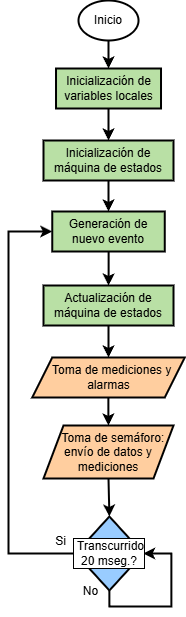
\includegraphics[width=0.4\textwidth]{./Figures/flowTaskApp.png}
\caption{Diagrama de flujo de la tarea del backend.}
\label{fig:taskApp}
\end{figure}

\subsection{Tarea del frontend}

El proceso del frontend ejecuta de forma cíclica el refresco de la pantalla LCD, es decir, dibuja la pantalla en su totalidad coloreando los píxeles. A bajo nivel, esto significa escribir el registro de la memoria asociado a cada píxel con un valor que corresponde a un color determinado. 

Debido a la cantidad de píxeles de la pantalla LCD y el tiempo que le toma al programa actualizarla en su totalidad, se decidió actualizarla a una tasa de diez veces por segundo (cada 0,1 seg.). Teniendo en cuenta que en esta aplicación los eventos visibles ocurren a baja velocidad, aumentar la tasa de muestreo no aportaría una mejora significativa. En cuanto a las variables medidas, para poder ser legibles, sus valores se actualizan solamente dos veces por segundo.

El proceso de refresco comienza cuando la tarea toma el semáforo que le permite acceder a la variable compartida con el proceso de backend. El frontend copia los valores localmente y libera el semáforo. Luego realiza la actualización de toda la pantalla con los valores obtenidos, a excepción de las mediciones analógicas.

A continuación el programa verifica si ya transcurrió medio segundo desde la ultima actualización de los valores analógicos. En caso afirmativo, realiza el mismo proceso que antes pero con los valores de las mediciones. Si no pasó dicho tiempo, continúa y espera que trascurra 0,1 segundo antes de realizar la próxima actualización de la pantalla.

En la figura \ref{fig:taskDisp} se puede ver un diagrama de flujo general de la tarea de frontend.

\begin{figure}[H]
\centering
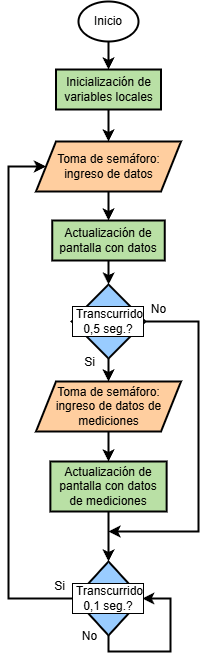
\includegraphics[width=0.4\textwidth]{./Figures/flowTaskDisp.png}
\caption{Diagrama de flujo de la tarea del frontend.}
\label{fig:taskDisp}
\end{figure}

\subsection{Máquina de estados}
\subsubsection{Diseño}

La máquina de estados implementada administra el funcionamiento del amplificador en todo momento mediante su interfaz eléctrica y el control de la alimentación. Cada uno de los estados de la máquina describen de forma análoga el estado real del EDFA. En base a los requerimientos se han definido los siguientes:

\begin{itemize}
\item Desconectado: alimentación del amplificador desconectada (relé desactivado y valor de tensión válido).
\item Conectado: amplificador energizado (relé activado).
\item Activo: salida óptica del amplificador encendida.
\item Alimentación fuera de rango: valor de la alimentación del EDFA fuera del rango permitido.
\item Alarma encendida: alarma del EDFA encendida (cualquiera de ellas).
\end{itemize}

Todas las posibles transiciones entre estos estados son disparadas por eventos que pueden ocurrir en cualquier momento, y ejecutan una acción según el estado en que se encuentre la máquina. La cantidad de eventos que pueden llegar a la máquina es elevada, por lo que, por simplicidad solo se mencionan algunos a modo de ejemplo:

\begin{itemize}
\item Eventos de la alimentación: baja tensión, sobretensión y sobrecorriente.
\item Eventos de la pantalla táctil: botón de encendido presionado, botón de apagado presionado, etc.
\item Eventos del amplificador: alarma de potencia de entrada encendida, potencia óptica de salida excedida, etc.
\item Eventos de la consola de control: comando de conexión de alimentación recibido, comando de encendido de salida del amplificador recibido, comando inválido, etc.
\end{itemize}

En la figura \ref{fig:diagFSM} se puede ver un diagrama simplificado de transiciones de la máquina de estados implementada, que incluye sus estados y eventos asociados.

\begin{figure}[H]
\centering
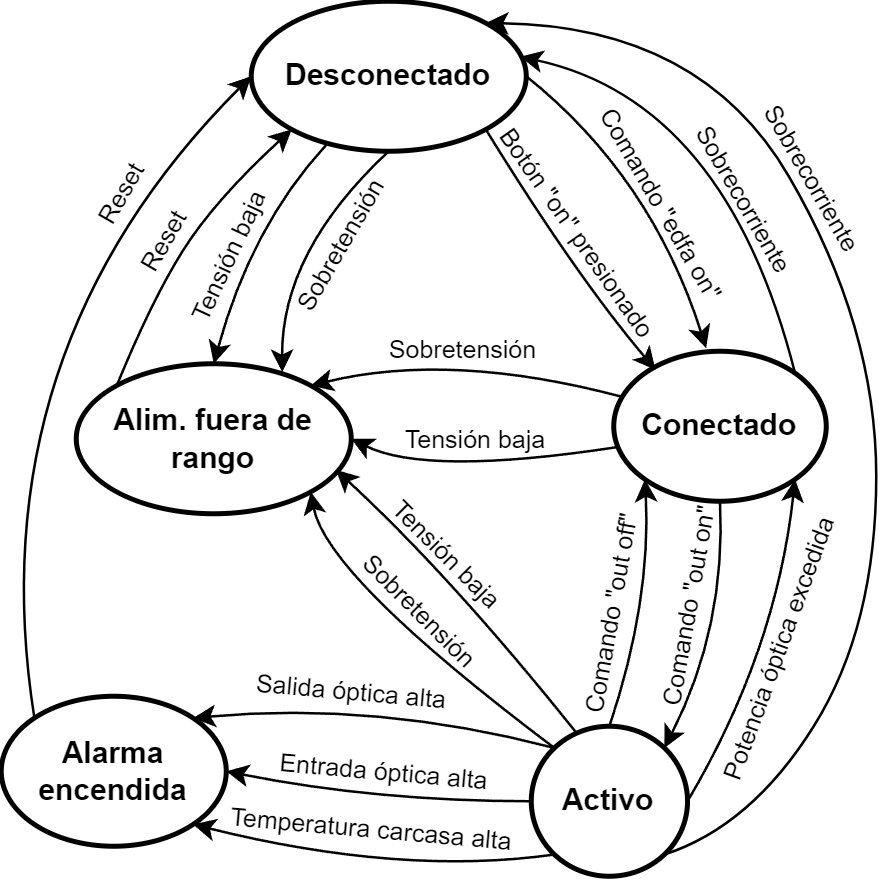
\includegraphics[width=0.85\textwidth]{./Figures/diagFSM.png}
\caption{Diagrama simplificado de la máquina de estados.}
\label{fig:diagFSM}
\end{figure}

\subsubsection{Implementación}

Para implementar de forma conveniente la máquina de estados lo que se hizo fue usar el tipo de dato que se ve en la figura \ref{fig:typeFSM}.

\begin{figure}[H]
\centering
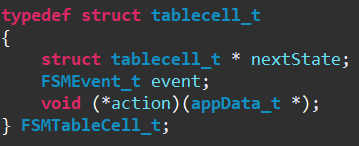
\includegraphics[width=0.6\textwidth]{./Figures/typeFSM.png}
\caption{Tipo de dato de la máquina de estados.}
\label{fig:typeFSM}
\end{figure}

Si se interpreta a la máquina de estados como una tabla de doble entrada, donde los eventos se colocan en las columnas y los estados en las filas, cada intersección representa la función a ejecutar cuando se da una transición. Este tipo de dato contiene tres variables y representaría una celda de dicha tabla:

\begin{itemize}
\item \textbf{nextState}: puntero a otra variable del mismo tipo. Indica el próximo estado de la máquina luego de ejecutar la función.
\item \textbf{event}: evento definido en una lista con todos posibles. Indica bajo que evento se ejecutará la función apuntada por esta celda.
\item \textbf{action}: puntero a función. Apunta a la función a ejecutar propiamente dicha.
\end{itemize}

Por lo tanto, si se define un arreglo de este tipo de dato para cada uno de los estados de la máquina y se lo llena con la cantidad de elementos correspondientes a cada posible transición, se cuenta con una representación completa de toda la máquina.

\subsection{Capa de abstracción del amplificador}
\label{sec:secHAL}

Con el objetivo de generar una estructura jerárquica, se decidió crear una capa adicional que se ubica por encima de los drivers de la pantalla LCD, de la pantalla táctil, de la UART, de las señales analógicas y de los GPIO provistos por la HAL del fabricante (ST). A su vez, los drivers de la pantalla LCD y la pantalla táctil se implementan con base en el driver de SPI, ya que debe hacer uso de las funciones de bajo nivel para el envío y recepción de datos y comandos. Para el ADC también se creó una pequeña capa superior que permite obtener todos los valores de las señales analógicas en formato de punto flotante.

De esta forma se genera un nivel más de abstracción que provee un conjunto de funciones o servicios para interactuar con el EDFA, funcionando a modo de puente entre este y la aplicación de usuario (backend). En la figura \ref{fig:halAmp} se puede ver la estructura de esta capa junto con sus distintos niveles.

\begin{figure}[H]
\centering
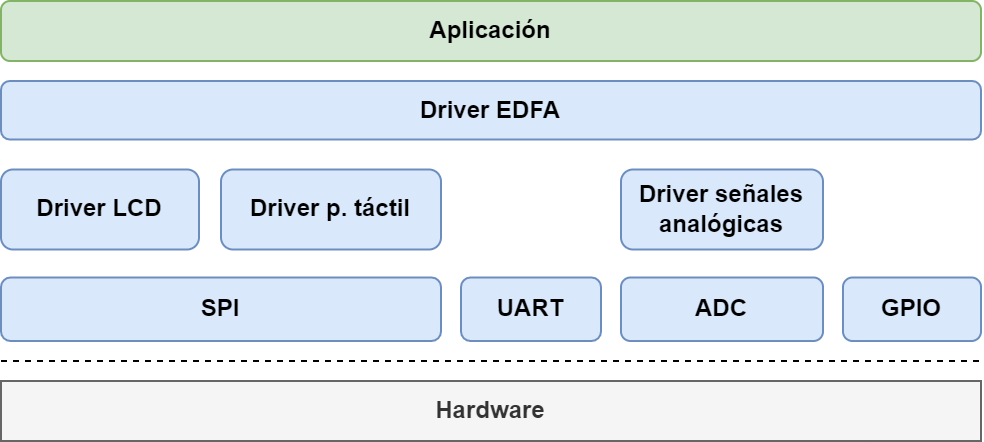
\includegraphics[width=0.9\textwidth]{./Figures/halamp2.png}
\caption{Capa de abstracción del EDFA.}
\label{fig:halAmp}
\end{figure}

\subsection{Driver del ADC}

Para la lectura de los valores analógicos se decidió utilizar el driver del ADC mediante DMA. Esto trae la principal ventaja de que solo se necesita realizar la configuración del ADC una sola vez al comienzo del programa y luego el muestreo y la conversión de los valores se realizará automáticamente de forma periódica.

En este caso esta implementación es particularmente útil debido a que se evita ocupar al procesador realizando la conversión manualmente y se puede atender a otras tareas. De esta forma, como el movimiento del dato convertido desde el periférico a la memoria se hace de forma automática, cuando el programa requiere leer el dato del valor convertido este ya se encuentra disponible en memoria.

Para filtrar ruido y posibles valores espurios que tome la señal analógica se aplica un pequeño filtro promediando 10 muestras continuas en cada canal usado. La configuración completa del ADC se muestra en la tabla \ref{tab:configADC}.

\begin{table}[H]
	\centering
	\caption{Configuración del ADC.}
	\begin{tabular}{l c}
		\toprule
		\textbf{Parámetro} & \textbf{Configuración}  \\
		\midrule
		Cantidad de canales usados & 4		\\
		Cantidad de bits		& 12 bits 	 		 \\
		Modo de conversión		& Continua   \\
		Tasa de muestreo		& 600 ksps	 \\
		Cantidad de muestras promediadas	& 10 \\
		Disparo de conversión	& Por software \\
		\bottomrule
		\hline
	\end{tabular}
	\label{tab:configADC}
\end{table}

Dado que el ADC opera con 12 bits y la tensión de referencia del microcontrolador es de 3,3 V, se obtienen 4096 niveles discretos (de 0 a 4095), lo que resulta en una resolución de aproximadamente 0,8 mV por cada bit menos significativo.

\subsection{Driver de la pantalla LCD}

Como se mencionó en la sección \ref{sec:conLCD}, cada bus SPI (LCD y pantalla táctil) tiene una interfaz dedicada en el microcontrolador funcionando este en modo maestro. La tabla \ref{tab:configSPI} muestra un resumen de la configuración de ambos controladores.

\begin{table}[H]
	\centering
	\caption{Configuración de los SPI del LCD.}
	\begin{tabular}{l c c}
		\toprule
		\textbf{Parámetro} & \textbf{LCD} & \textbf{Pantalla táctil} \\
		\midrule
		Velocidad de transmisión	& 8 Mbps & 4 Mbps	\\
		Ancho de palabra 				& 8 bits & 8 bits	    \\
		Polaridad							& Baja & Baja \\
		Dirección							& Bidireccional & Bidireccional \\
		\bottomrule
		\hline
	\end{tabular}
	\label{tab:configSPI}
\end{table}

Como se mencionó en la sección \ref{sec:secHAL}, este driver está implementado sobre el de SPI. A su vez, las funciones que contiene también tienen cierta jerarquía entre si, permitiendo hacer funciones complejas usando otras más básicas. Tomando como ejemplo la función para dibujar un cuadrado sin relleno de color se tienen, de mayor a menor abstracción, las siguientes funciones:

\begin{itemize}
\item \textbf{LCD\_Draw\_Hollow\_Rectangle\_Coord}: recibe 2 pares de coordenadas para los vértices y el color. Llama 2 veces a la función que dibuja una línea horizontal y dos veces a la que dibuja una línea vertical, con la coordenada de origen y el largo correspondiente.
\item \textbf{LCD\_Draw\_Horizontal\_Line}: recibe la coordenada de origen, el largo y el color de la línea. Llama a la función que define la sección de la memoria del chip asociada a los píxeles a dibujar. Luego llama a la función que transmite el color a esta sección de memoria.
\item \textbf{LCD\_Draw\_Colour\_Burst}: transmite el color de los píxeles llamando a la función de transmisión de datos del SPI.
\item \textbf{LCD\_Set\_Address}: envía los comandos y direcciones de registros para definir la zona de memoria a escribir.
\item \textbf{LCD\_Write\_Data}: envía el dato recibido llamando a la función de transmisión de datos del SPI. Pone la señal DC del chip del LCD en alto, indicando que el valor transmitido es un dato.
\item \textbf{LCD\_Write\_Command}: envía el comando recibido llamando a la función de transmisión de datos del SPI. Pone la señal DC del chip del LCD en bajo, indicando que el valor transmitido es un comando.
\end{itemize}

\subsection{Driver de UART}

El controlador de UART para ambas interfaces se configura de modo que genere una interrupción en el programa luego de recibir una cadena de caracteres. Esto funciona de forma que los caracteres que se reciben se guardan continuamente en un buffer de entrada hasta que la línea de datos pasa a estar inactiva. Luego se atiende la interrupción y en ella se copia al programa principal la cadena de caracteres del buffer para ser analizada.

En la tabla \ref{tab:configUART} se puede ver la configuración de ambas interfaces UART.

\begin{table}[H]
	\centering
	\caption{Configuración de la interfaz UART.}
	\begin{tabular}{l c}
		\toprule
		\textbf{Parámetro} & \textbf{Configuración} \\
		\midrule
		Velocidad de transmisión	& 115200 baudios \\
		Ancho de palabra 				& 8 bits \\
		Bits de stop						& 1 bit \\
		Paridad							    & Ninguna \\
		Control de hardware			& Ninguno \\
		\bottomrule
		\hline
	\end{tabular}
	\label{tab:configUART}
\end{table}

\subsection{Consola de control}

%habria que mencionar en alguno de las primeras secciones la existencia de la consola de control

La consola de control brinda una pequeña interfaz que funciona como intermediario entre el usuario y el amplificador, permitiéndole consultar y controlar su estado en todo momento. También se utiliza para ingresar valores al dispositivo, tales como los niveles de tensión y corriente máximos admitidos.

Las funciones de la consola se ejecutan en la tarea del backend, puede inyectar eventos a la máquina de estados y utiliza el bus USB-UART para el flujo de caracteres. Su funcionamiento es similar al de cualquier consola o línea de comando y se basa en el ingreso de comandos en formato instrucción/argumento.

Su funcionamiento básico es el siguiente: luego de recibir una cadena de caracteres por UART y recuperarla en el backend, como se explicó en la subsección anterior, esta se pasa por lo que se denomina un \textit{parser}. Este lo que hace es primero identificar los caracteres de espacio que contiene la cadena para delimitar y extraer los comandos y argumentos (subcadenas). A continuación, se verifica si el comando ingresado coincide con alguno de los comandos válidos mediante la comparación de cadenas. En caso que este sea válido, se pasa a evaluar el argumento en base al tipo de dato que espera el comando. Por ejemplo, si el comando espera un número positivo se verifica que la cadena no contenga letras, que el valor sea positivo y que se encuentre dentro de los valores máximos y mínimos.

Si ambos comando y argumento son válidos entonces el programa generará el evento correspondiente a ese comando para luego ingresar a la máquina de estados. En caso que alguno no lo sea, ya sea por error de sintaxis o de argumento fuera de rango, no se generará ningún evento y la consola imprimirá "Comando inválido".

En la figura \ref{fig:flowCmd} se puede ver el diagrama de flujo desde que se recibe la cadena de caracteres en el buffer de la UART hasta la generación del evento correspondiente.

\begin{figure}[H]
\centering
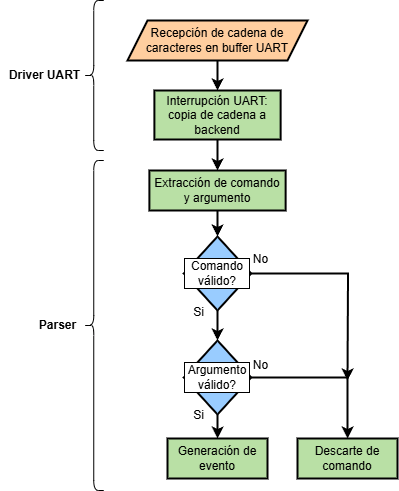
\includegraphics[width=0.75\textwidth]{./Figures/flowCmd.png}
\caption{Diagrama de flujo de la consola de control.}
\label{fig:flowCmd}
\end{figure}

La tabla \ref{tab:tablacmd} lista todos los pares comando/argumento que puede recibir la consola.

\begin{table}[H]
	\centering
	\caption{Comandos/argumentos de la consola.}
	\begin{tabular}{l c p{8cm}}
		\toprule
		\textbf{Comando} & \textbf{Argumento} & \textbf{Descripción} \\
		\midrule
		edfa	& on & Conecta la alimentación del EDFA.	\\
		edfa	& off & Desconecta la alimentación del EDFA. \\
		out	& on & Prende la salida óptica del EDFA. \\
		out   & off & Apaga la salida óptica del EDFA. \\
		status & - & Indica el estado general del EDFA y los valores de las variables. \\
		reset & - & Envía la señal de reset al microcontrolador del EDFA. \\
		ilim	& (valor) & Establece el límite de corriente al valor del argumento. \\
		vul	& (valor) & Establece el límite superior de tensión al valor del argumento. \\
		vll		& (valor) & Establece el límite inferior de tensión al valor del argumento. \\
		oipl	& (valor) & Establece el límite de potencia de entrada al valor del argumento. \\
		oopl & (valor) & Establece el límite de potencia de salida al valor del argumento. \\
		\bottomrule
		\hline
	\end{tabular}
	\label{tab:tablacmd}
\end{table}

\section{Dispositivo implementado}
\label{sec:dispImp}

Es importante aclarar que el dispositivo que se desarrolló e integró como solución a lo planteado en el capítulo 1 no es el producto final destinado a ser utilizado. La placa construida se puede interpretar como un prototipo de desarrollo o una versión de ingeniería, ya que cumple con dos objetivos principales: verificar el funcionamiento del hardware diseñado y desarrollar el firmware que se ejecutará en el microcontrolador. 

La versión armada para este trabajo, incluye los mismos componentes previstos para el producto final y, además, incorpora el hardware necesario para emular la interfaz electrónica del modelo del amplificador óptico, lo que permite generar todas las señales del conector, tanto analógicas como digitales.

Una vez alcanzados estos objetivos, la siguiente etapa consiste en desarrollar la placa del producto final, con el factor de forma adecuado para integrar y montar todos los componentes en una carcasa transportable. 

El PCB fue enviado a fabricar a la empresa china JLCPCB y consta de 4 capas: dos planos internos de referencia conectados a 3,3 V y GND y dos capas de señal (\textit{Top} y \textit{Bottom}). En la figura \ref{fig:placa1} y \ref{fig:placa2} se pueden ver dos fotos del PCB ensamblado sin el display ni la placa NUCLEO conectados (lado superior y lado inferior respectivamente). Por último, en la figura \ref{fig:placa3} se puede ver la placa con ambos módulos conectados.

\begin{figure}[H]
     \centering
     \begin{subfigure}{\textwidth}
         \centering
         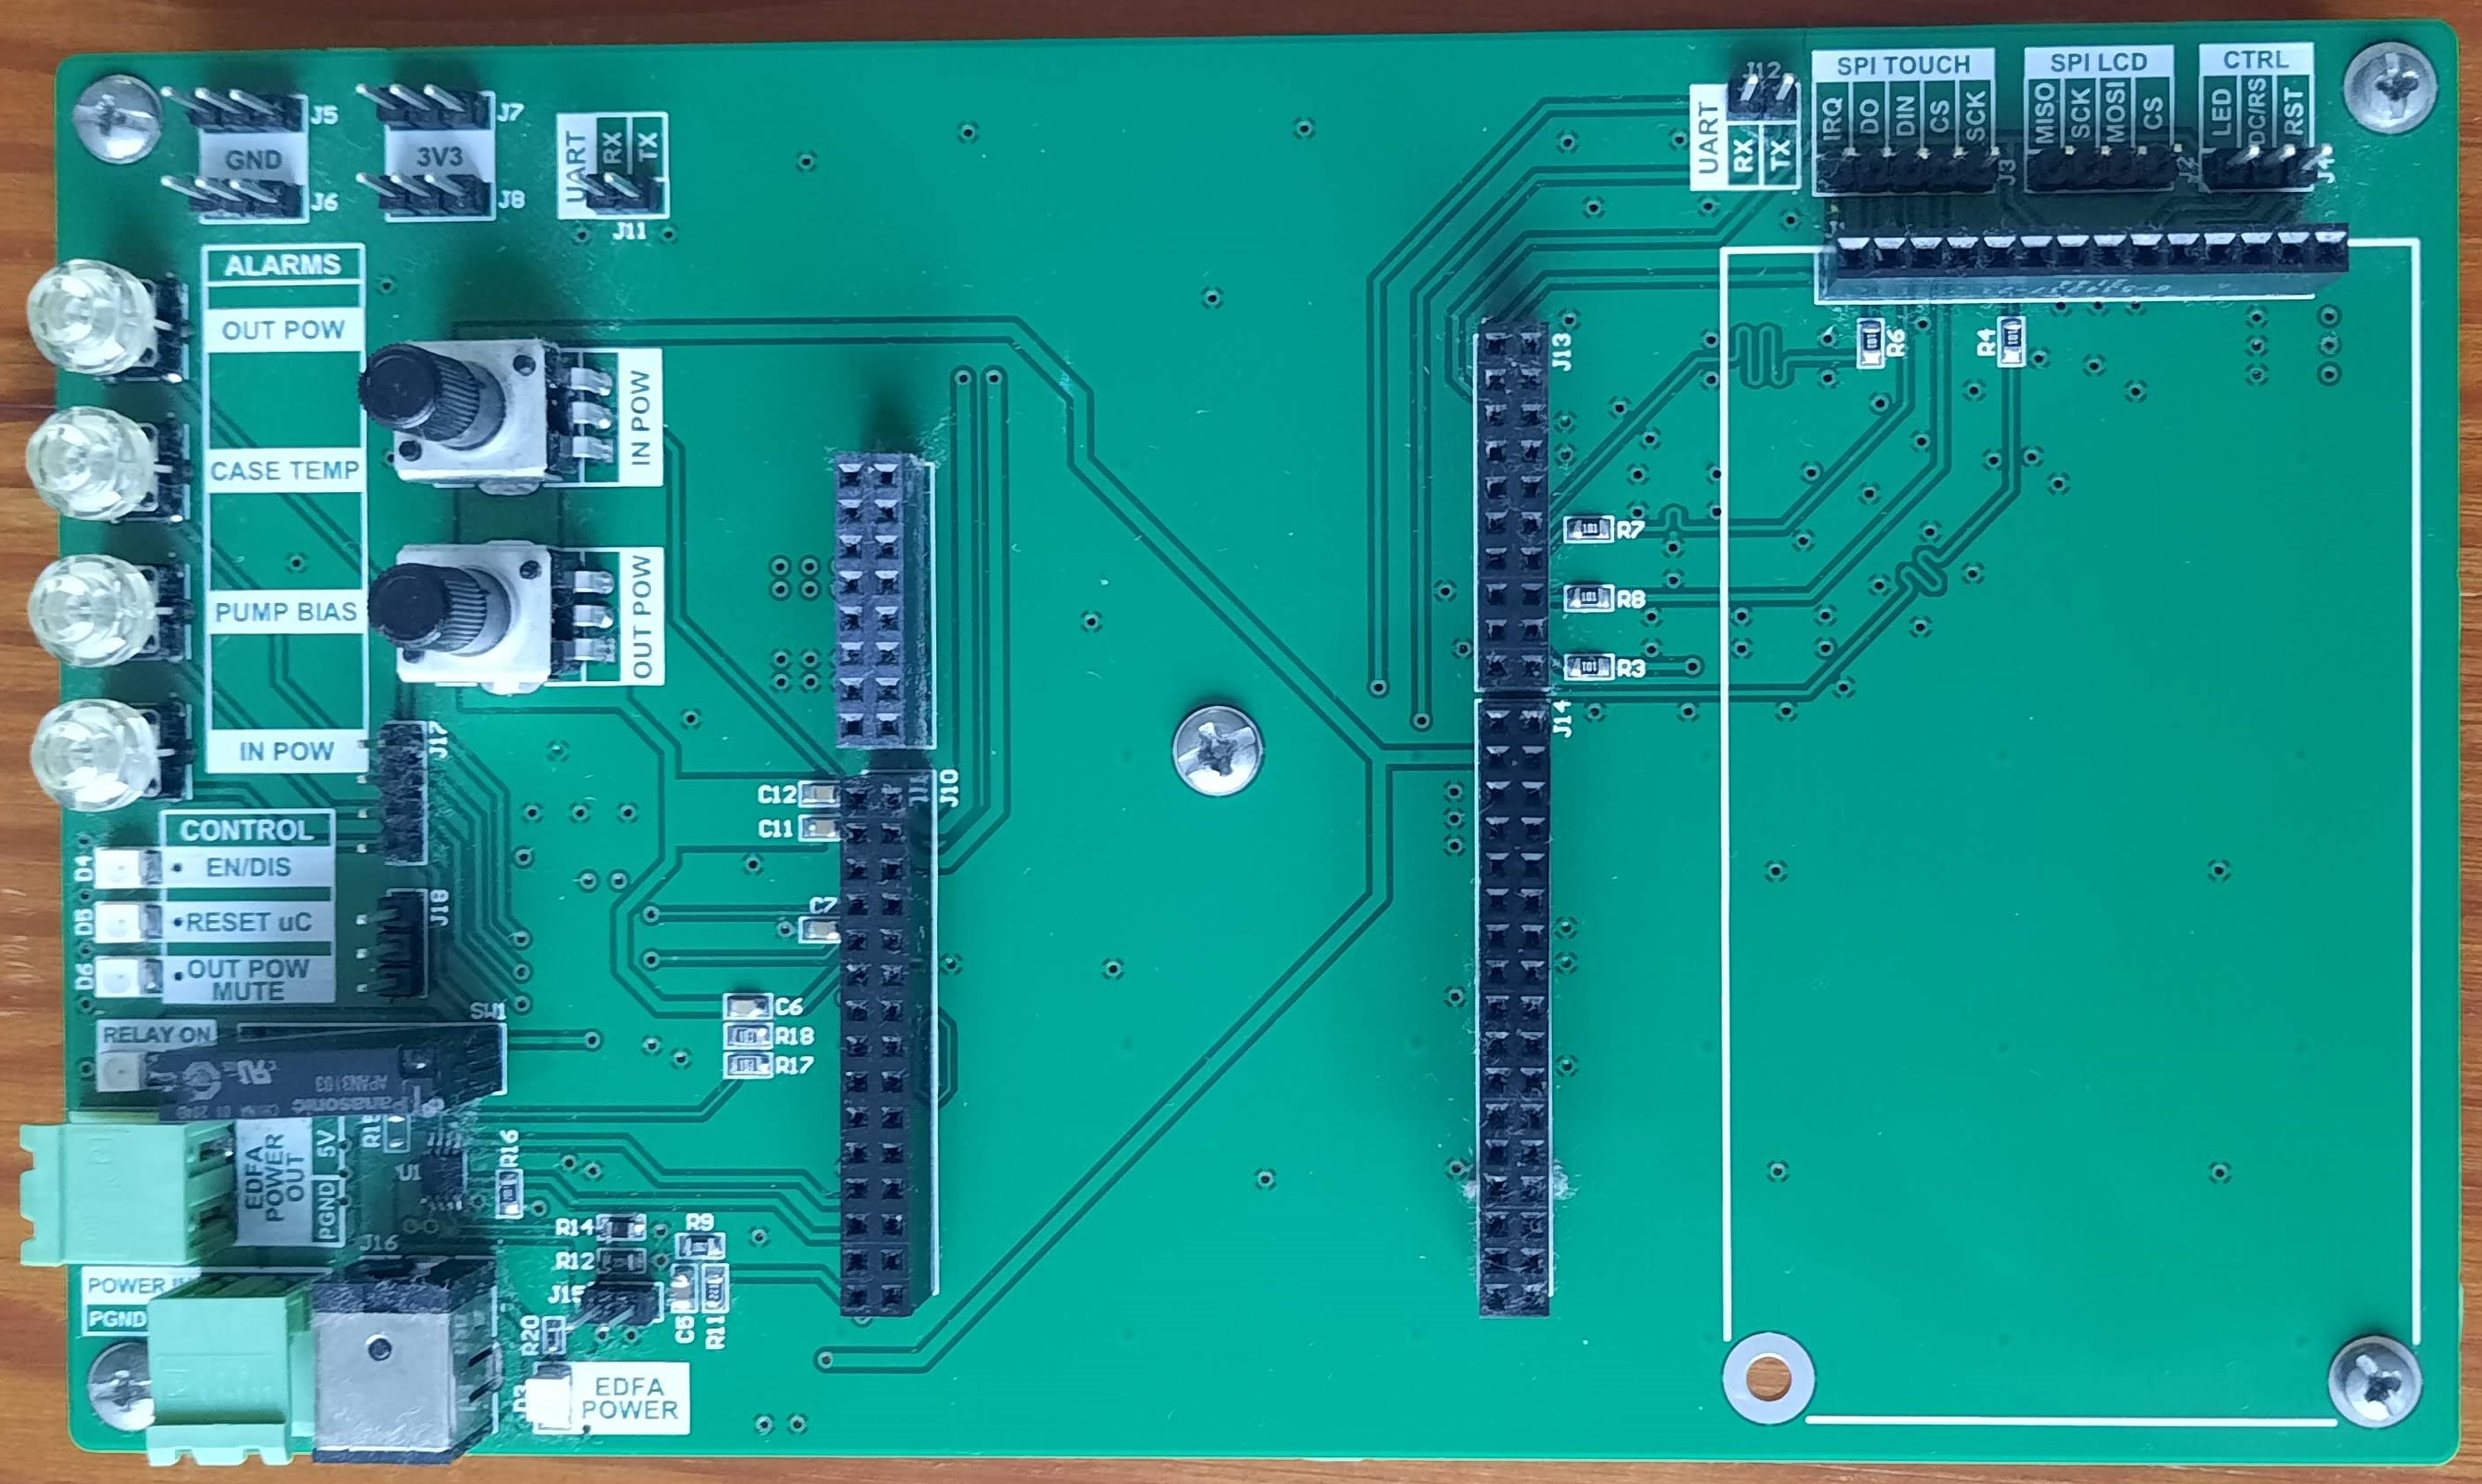
\includegraphics[width=.75\textwidth]{./Figures/placa2.jpg}
         \caption{Lado superior del PCB.}
         \label{fig:placa1}
     \end{subfigure}
     \begin{subfigure}{\textwidth}
         \centering
         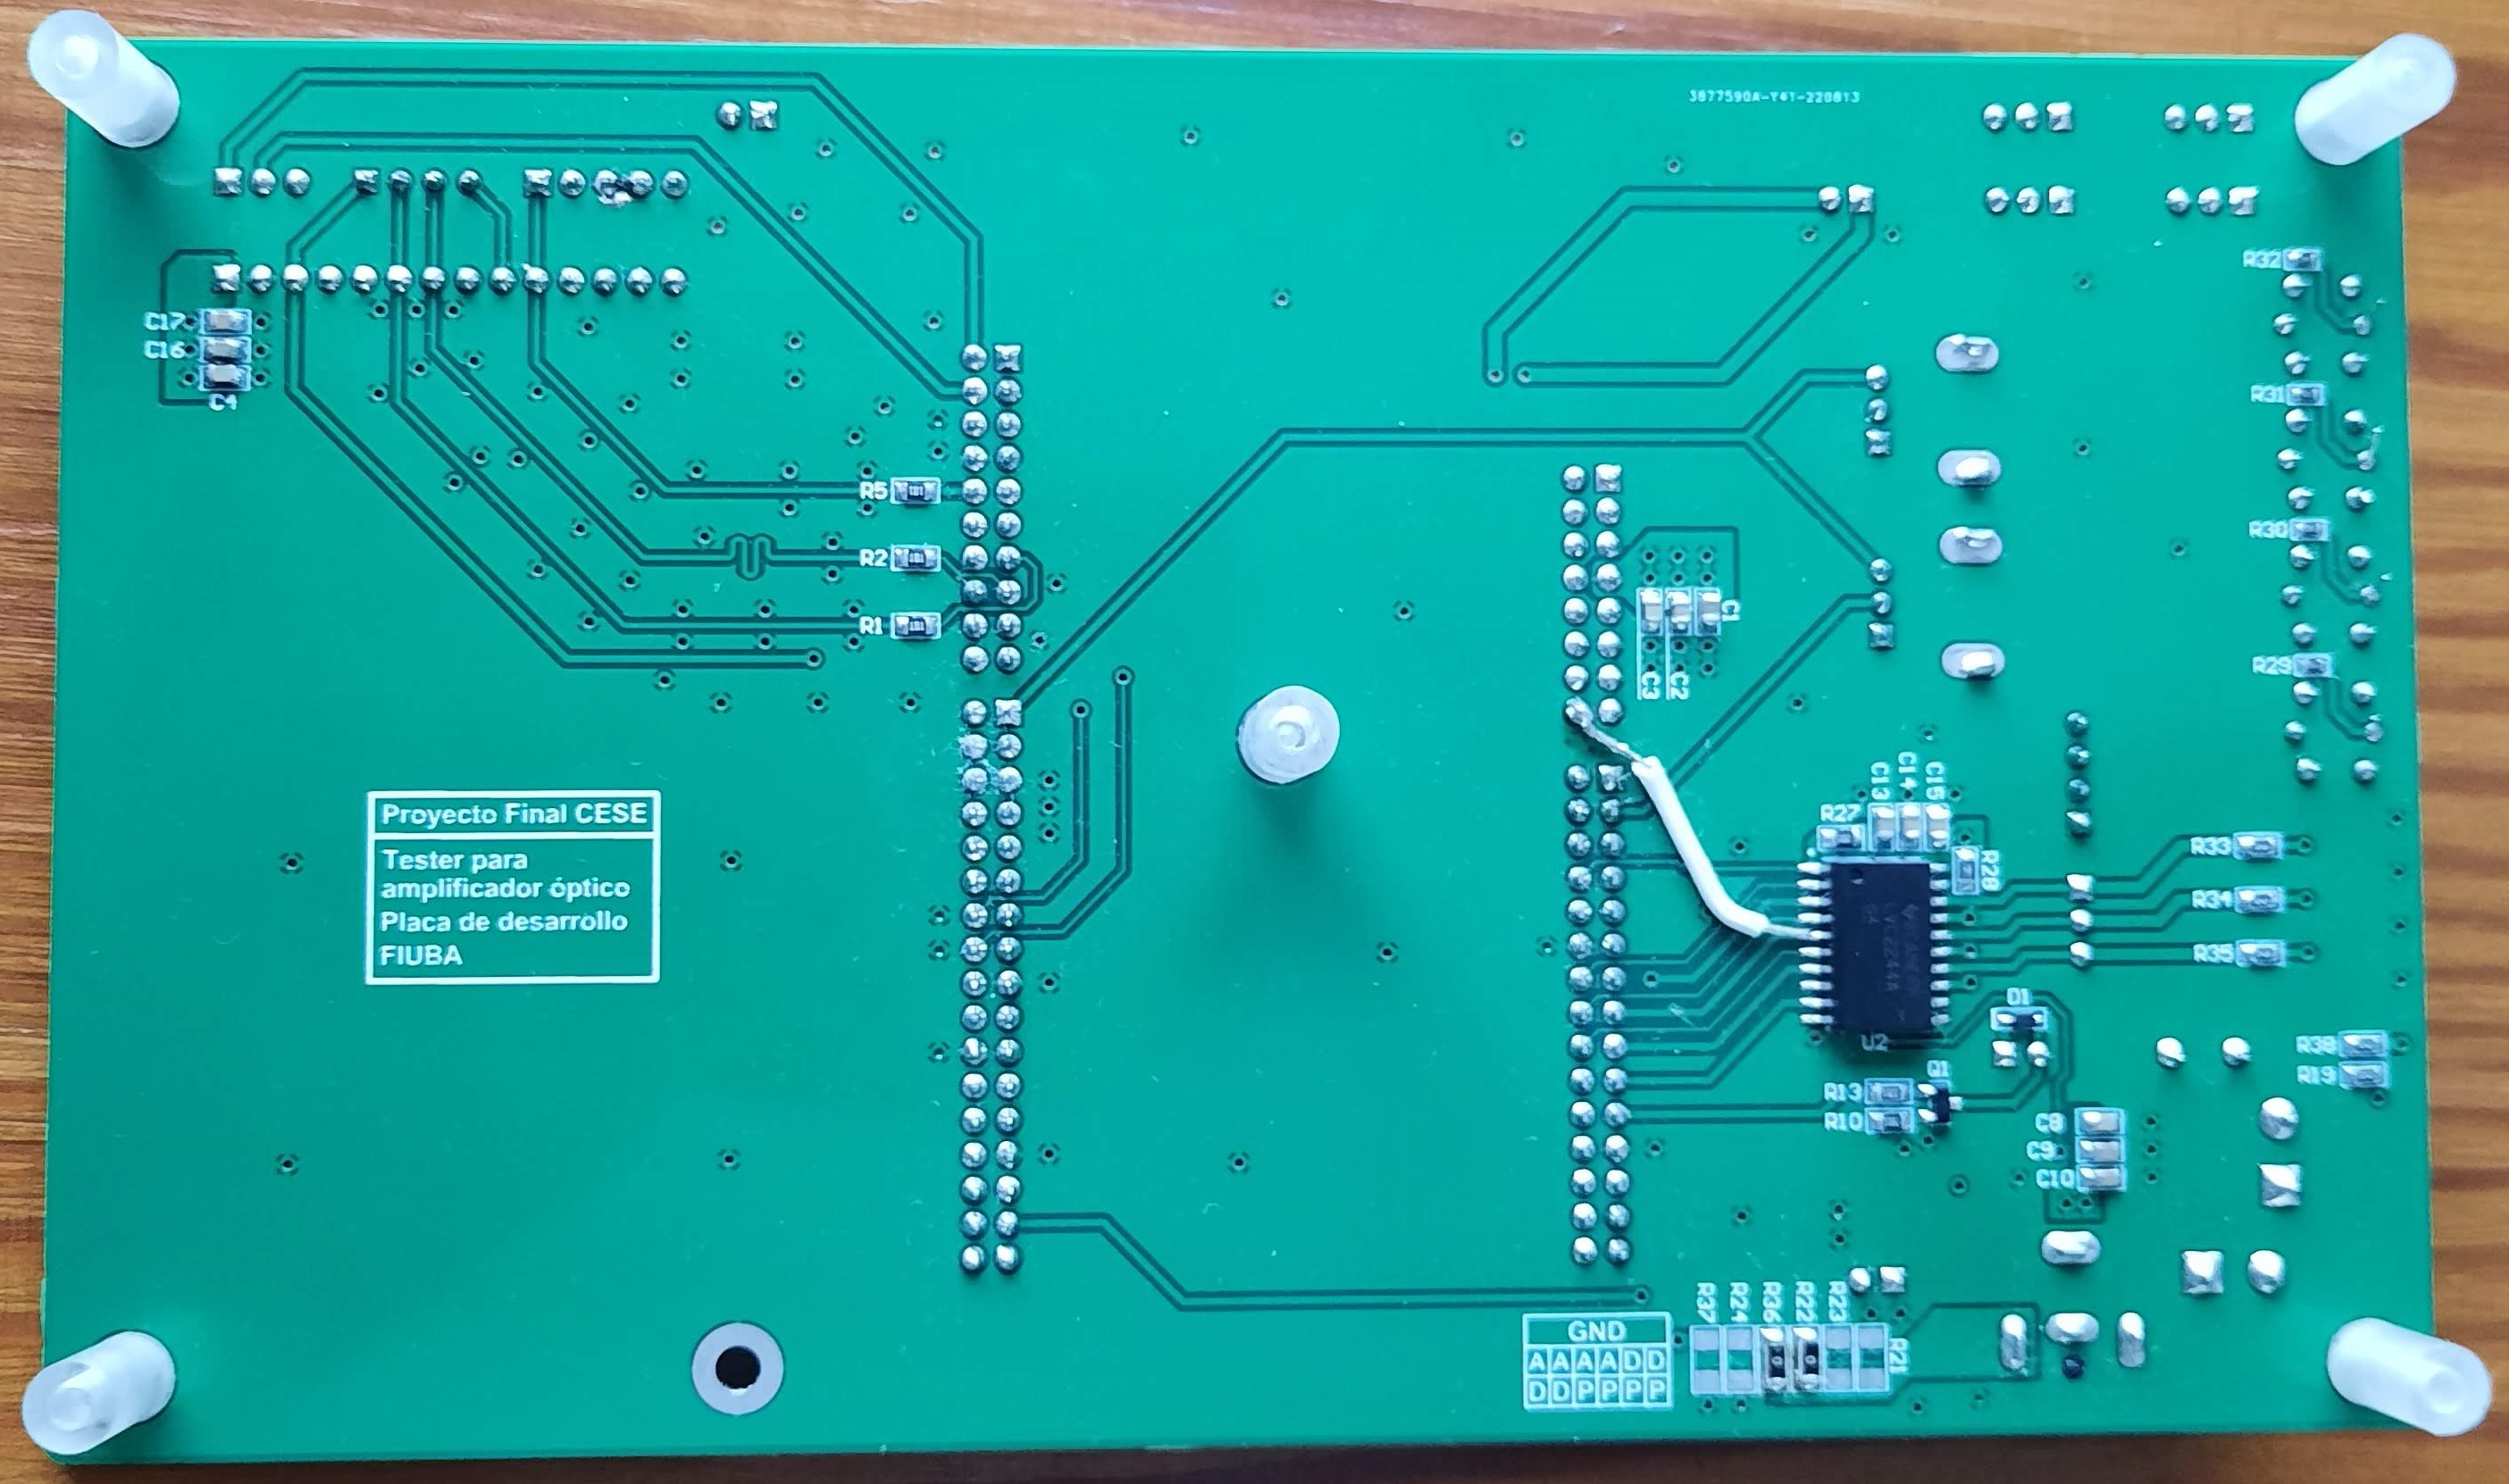
\includegraphics[width=.75\textwidth]{./Figures/placa3.jpg}
         \caption{Lado inferior del PCB.}
         \label{fig:placa2}
     \end{subfigure}
     \begin{subfigure}{\textwidth}
         \centering
         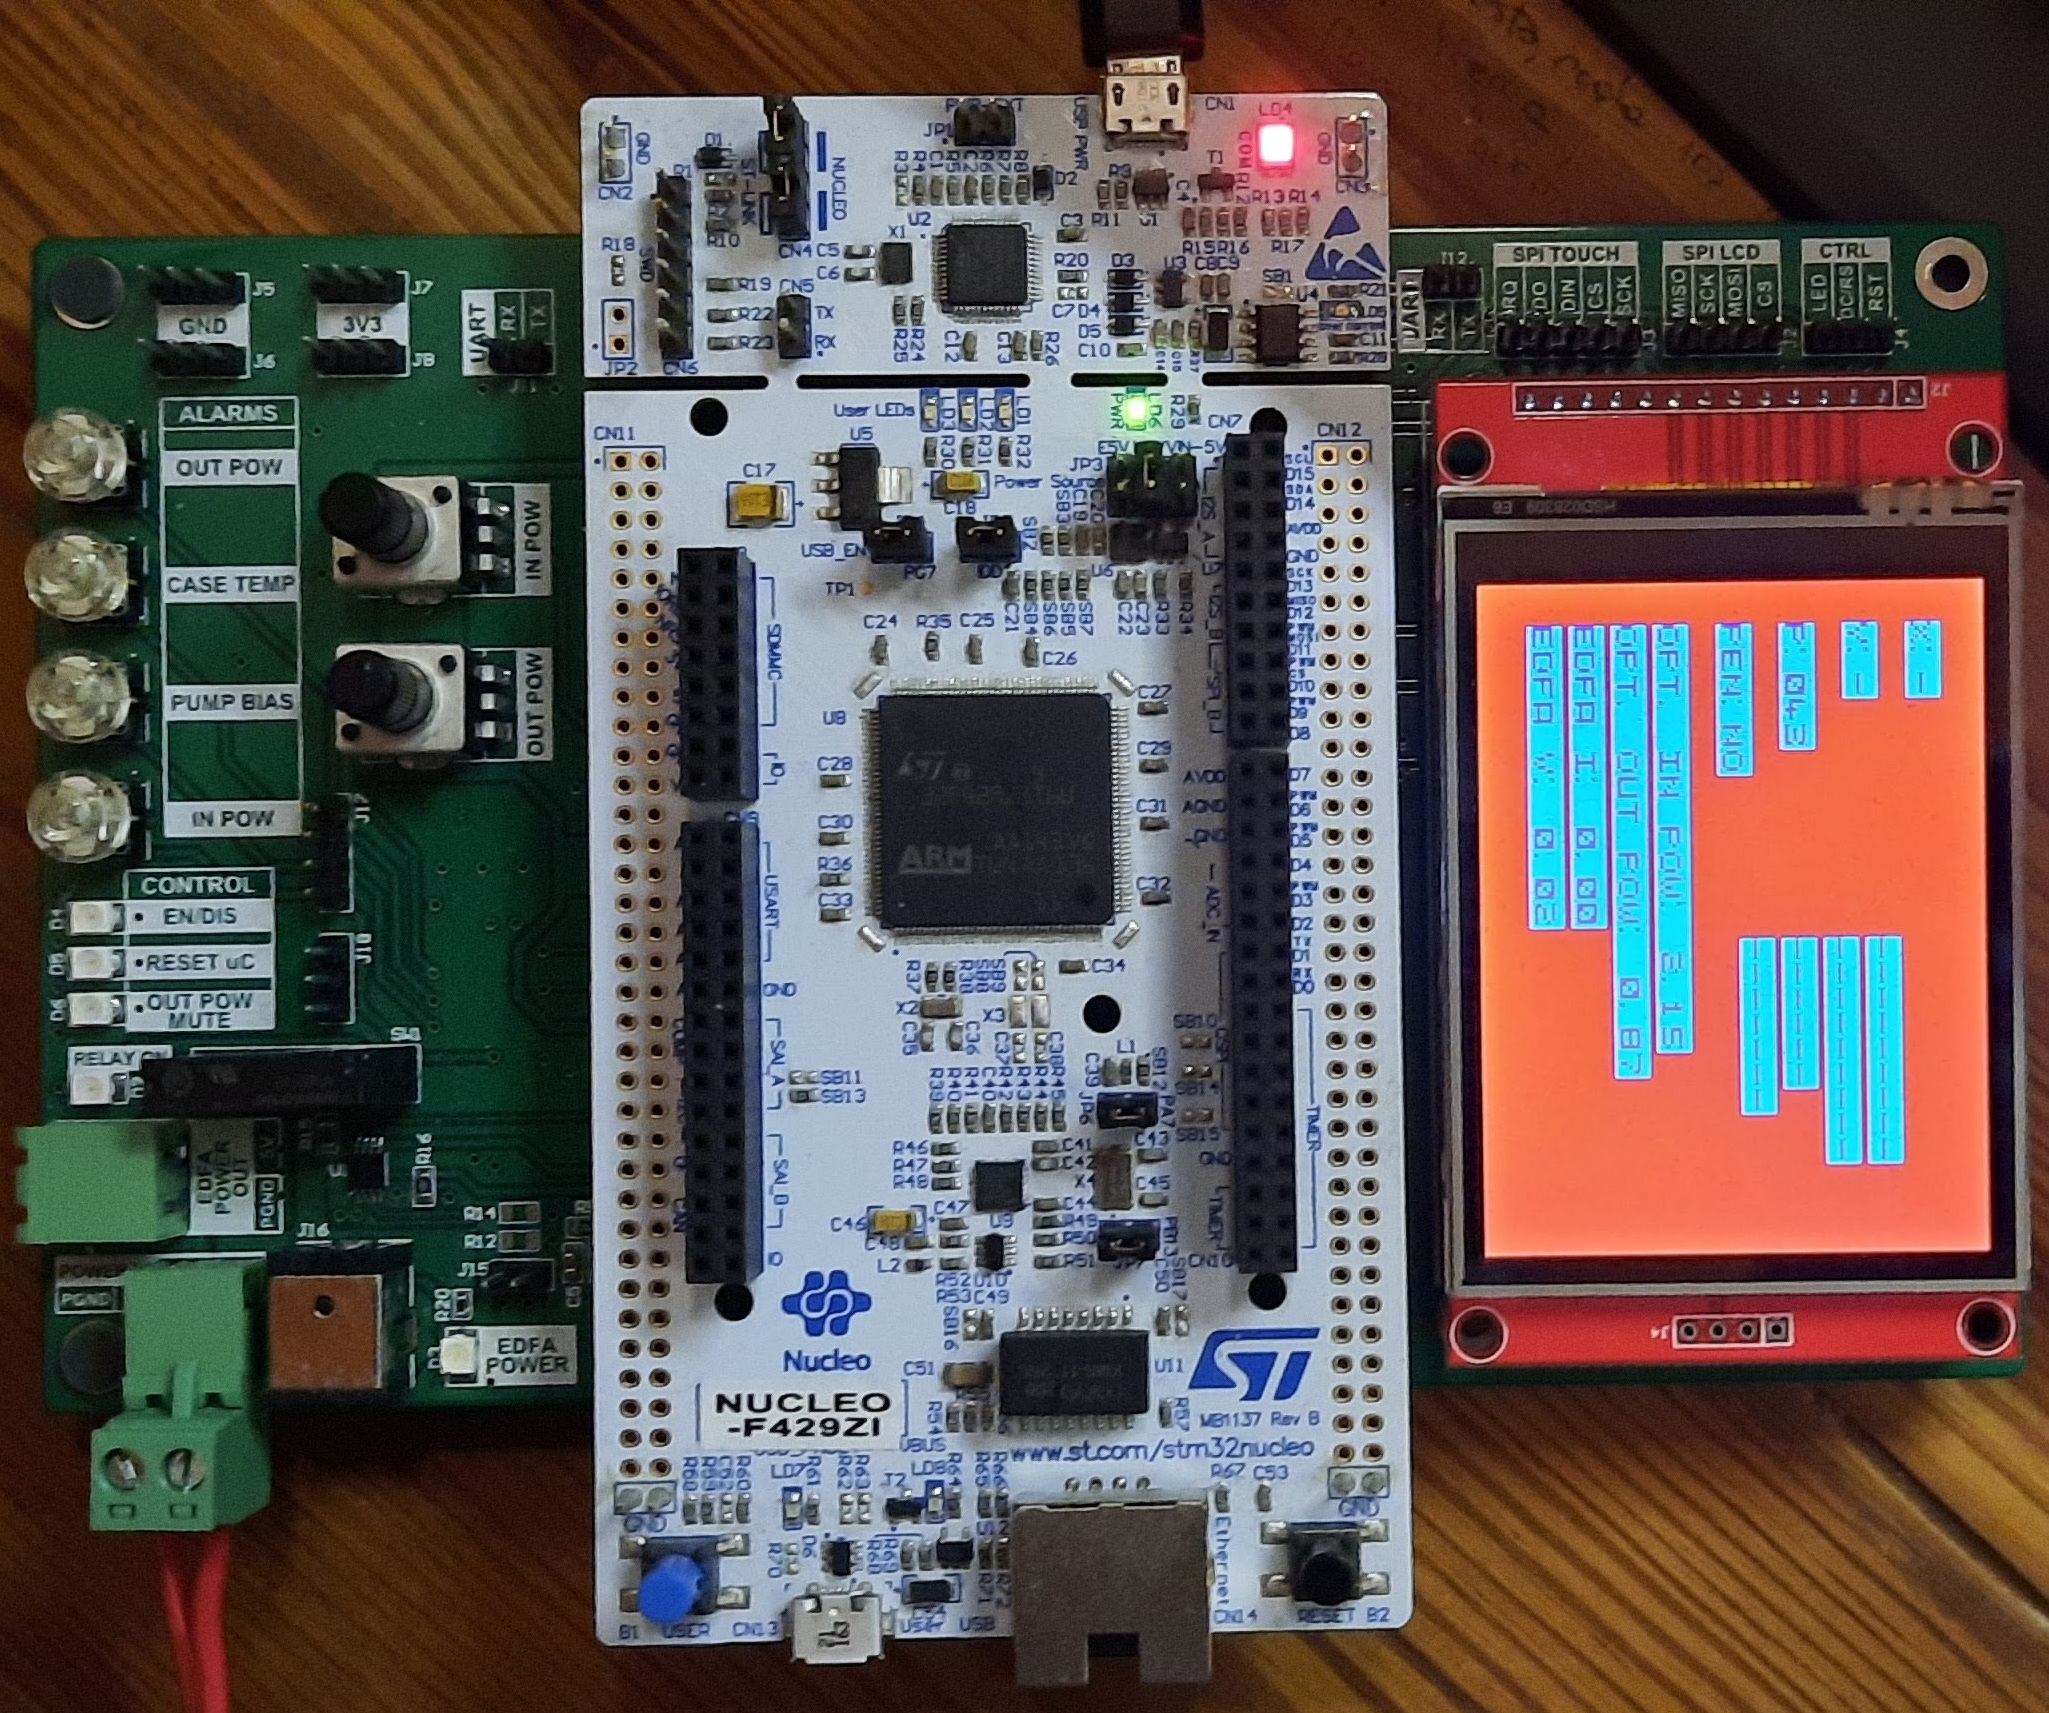
\includegraphics[width=.75\textwidth]{./Figures/placa1.jpg}
         \caption{Placa ensamblada.}
         \label{fig:placa3}
     \end{subfigure}
        \caption{Placa fabricada para el trabajo.}
        \label{fig:three graphs}
\end{figure}
% Chapter Template

\chapter{Ensayos y resultados} % Main chapter title

\label{Chapter4} % Change X to a consecutive number; for referencing this chapter elsewhere, use \ref{ChapterX}

%----------------------------------------------------------------------------------------
%	CHAPTER 4
%----------------------------------------------------------------------------------------

En este capítulo se explica cómo se llevaron a cabo las pruebas de validación de hardware y software a las que fue sometido el dispositivo, los bancos de ensayos, instrumentos utilizados y los resultados obtenidos.

\section{Instrumental utilizado}

Para poder ejecutar las pruebas de integración de hardware y software se requirió del uso de una variedad de instrumentos y componentes en los bancos de ensayos. La tabla \ref{tab:instrumentos} lista los detalles de cada uno de ellos.

\begin{table}[H]
	\centering
	\caption{Lista de instrumental utilizado.}
	\begin{tabular}{p{3cm} c p{6cm}}
		\toprule
		\textbf{Item} & \textbf{Modelo} & \textbf{Descripción} \\
		\midrule
		Multímetro			& UNI-T UT61A		& Multímetro digital autorango de alta precisión. \\
		Fuente de tensión	& KM GP-300ATX		& Fuente de computadora de 400 W. \\
		Resistencia de potencia variable		& AVT05006E25R00KE	& Resistencia de potencia de alambre bobinado de 25 Ohm / 50 W. \\
		Potenciómetro							& 3590S-1-201L & Potenciómetro de 200 Ohm / 2 W y 10 vueltas para panel. \\
		Conversor USB a UART					& EM7-6043		& Conversor USB a serie TTL CH-340. \\
		Cables varios							& - 			& Cables dupont y unipolar de 2,5 mm\textsuperscript{2}. \\
		PC										& -				& Computadora de escritorio con software PuTTY (cliente de terminal). \\
		\bottomrule
		\hline
	\end{tabular}
	\label{tab:instrumentos}
\end{table}

En el apéndice \ref{AppendixB} se puede ver una foto del banco de ensayos completo con todos los instrumentos y hardware utilizado.

\section{Pruebas de hardware}
\label{sec:pruebasHW}

Para validar el funcionamiento del hardware, basta con medir continuidad o niveles de tensión en ciertos puntos de la placa. Por esta razón, se omite especificar las pruebas a excepción de las del monitor de corriente, ya que es el único caso en el que es necesario realizar mediciones.

\subsection{Prueba del monitor de corriente}
\label{sec:monCorr}

En el circuito del monitor de corriente lo que se desea verificar es que a la salida del amplificador se obtenga una tensión proporcional al valor de corriente que circula. La constante de conversión surge de multiplicar el valor de la resistencia de sensado (10 mOhm) por la constante de amplificación del circuito integrado (100 V/V), lo que resulta en un valor de 1 V/A. Por lo tanto, la conversión entre corriente y tensión es unitaria.

Para realizar las mediciones se conecta la entrada de tensión a la fuente de 5 V, una resistencia de potencia en la salida de tensión y se varía su valor de forma de hacer circular desde 0 A hasta aproximadamente 3,3 A.

%\begin{figure}[H]
%\centering
%\includegraphics[width=0.9\textwidth]{./Figures/esqMonCorr.png}
%\caption{Esquema de medición del monitor de corriente.}
%\label{fig:esqMonCorr}
%\end{figure}

Con los datos obtenidos se calcula para cada medición el error porcentual con respecto al valor teórico de la constante de conversión. En la figura \ref{fig:testMonCorr} se pueden ver los valores computados para distintos valores de corriente en la carga.

\begin{figure}[H]
\centering
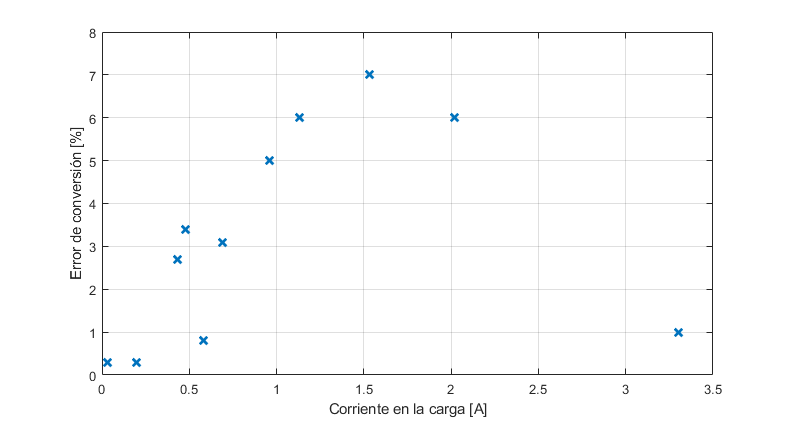
\includegraphics[width=0.9\textwidth]{./Figures/testMonCorr.png}
\caption{Error porcentual de la constante de conversión de corriente.}
\label{fig:testMonCorr}
\end{figure}

Del gráfico se observa que en este rango se tiene un error de medición máximo del 7 \% y un valor promedio aproximado del 3,23 \% respecto del valor real.

Esta diferencia entre el valor de la constante medida y el teórico se la puede atribuir principalmente a dos efectos: la dispersión del valor de la resistencia de sensado y a la presencia de ruido en el circuito. El error de la ganancia del circuito integrado está especificado en un máximo de 0,2\% por lo que no aporta variaciones significativas.

\section{Pruebas de firmware}
\label{sec:pruebasFW}

Las pruebas de firmware tienen como finalidad validar el funcionamiento individual de una biblioteca o una parte en particular del código desarrollado. Para ello, en algunos casos lo que se hace es directamente mostrar funcionalidades específicas del programa funcionando, como por ejemplo en el driver de la pantalla LCD y de la consola de control.

\subsection{Prueba del monitor de tensión}

Para el monitor de tensión y el monitor de corriente (siguiente subsección) se desea verificar que las mediciones se realizan con un error menor al especificado en el requerimiento 1.4, en la sección \ref{sec:reqs}.

Para realizar las mediciones se conecta la entrada de tensión a una fuente variable y se lee directamente el valor medido que muestra la pantalla LCD. Se toman valores en el rango entre 0 V y 5 V en pasos aproximados de 0,5 V.

Con el valor de tensión de entrada y el medido por la placa se computa el error para cada medición (con respecto al de tensión de entrada). En la figura \ref{fig:testMonTens} se pueden ver los valores computados para los distintos valores de tensión de entrada.

\begin{figure}[H]
\centering
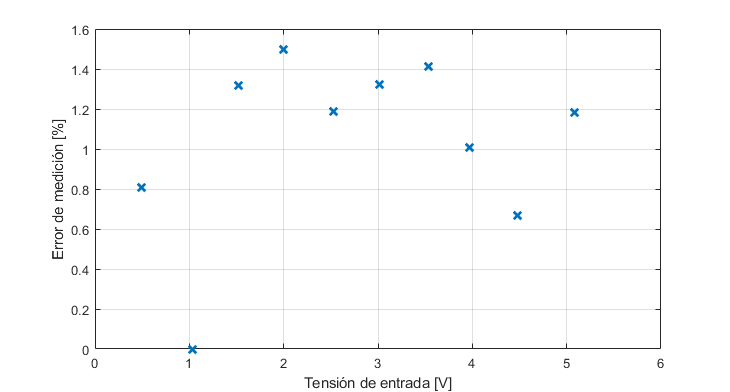
\includegraphics[width=0.9\textwidth]{./Figures/testMonTens.png}
\caption{Error porcentual de la medición de tensión.}
\label{fig:testMonTens}
\end{figure}

Del gráfico se observa que en este rango se tiene un error de medición máximo del 1,5 \% y un valor promedio aproximado del 1,04 \% respecto del valor real.

\subsection{Prueba del monitor de corriente}

Para esta prueba se procede de igual forma que en la subsección \ref{sec:monCorr} pero en lugar de medir la tensión de salida del monitor se toma directamente la lectura de medición de corriente de la pantalla LCD.

Con los datos obtenidos se calcula para cada medición el error porcentual con respecto al valor real de corriente de carga. En la figura \ref{fig:testMonCorr2} se pueden ver los valores computados para distintos valores de corriente en la carga.

\begin{figure}[H]
\centering
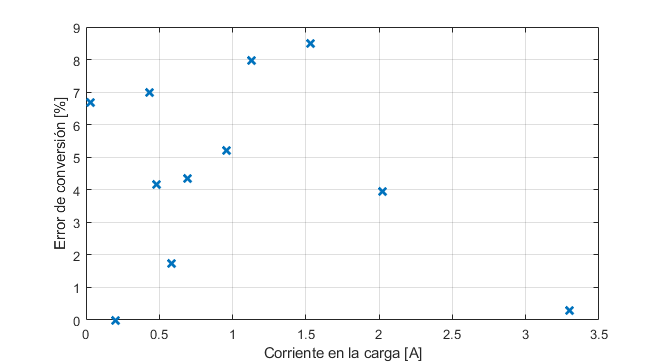
\includegraphics[width=0.9\textwidth]{./Figures/testMonCorr2.png}
\caption{Error porcentual de la medición de corriente.}
\label{fig:testMonCorr2}
\end{figure}

Observando el gráfico se desprende que en este rango se tiene un error de medición máximo del 8,5 \% y un valor promedio aproximado del 4,52 \% respecto del valor real. Estos valores resultan ligeramente mayores a los obtenidos en la sección \ref{sec:monCorr}, lo cual es de esperarse ya que durante el procesamiento digital de los datos se introduce más incerteza (debido a la resolución del ADC) y error de cálculo.

\subsection{Prueba de la pantalla LCD}

En este caso se muestra directamente el LCD durante el funcionamiento normal del programa, lo que implica no solo que la biblioteca desarrollada para la pantalla funciona, si no que los drivers del SPI sobre los que esta implementada también.

En la figura \ref{fig:testLCD} se puede ver la pantalla LCD durante el inicio del programa luego de encender la placa. Como se puede ver, contiene texto y rectángulos de distintos colores, lo que implica el uso de la mayoría de las funciones implementadas en la biblioteca.

\begin{figure}[H]
\centering
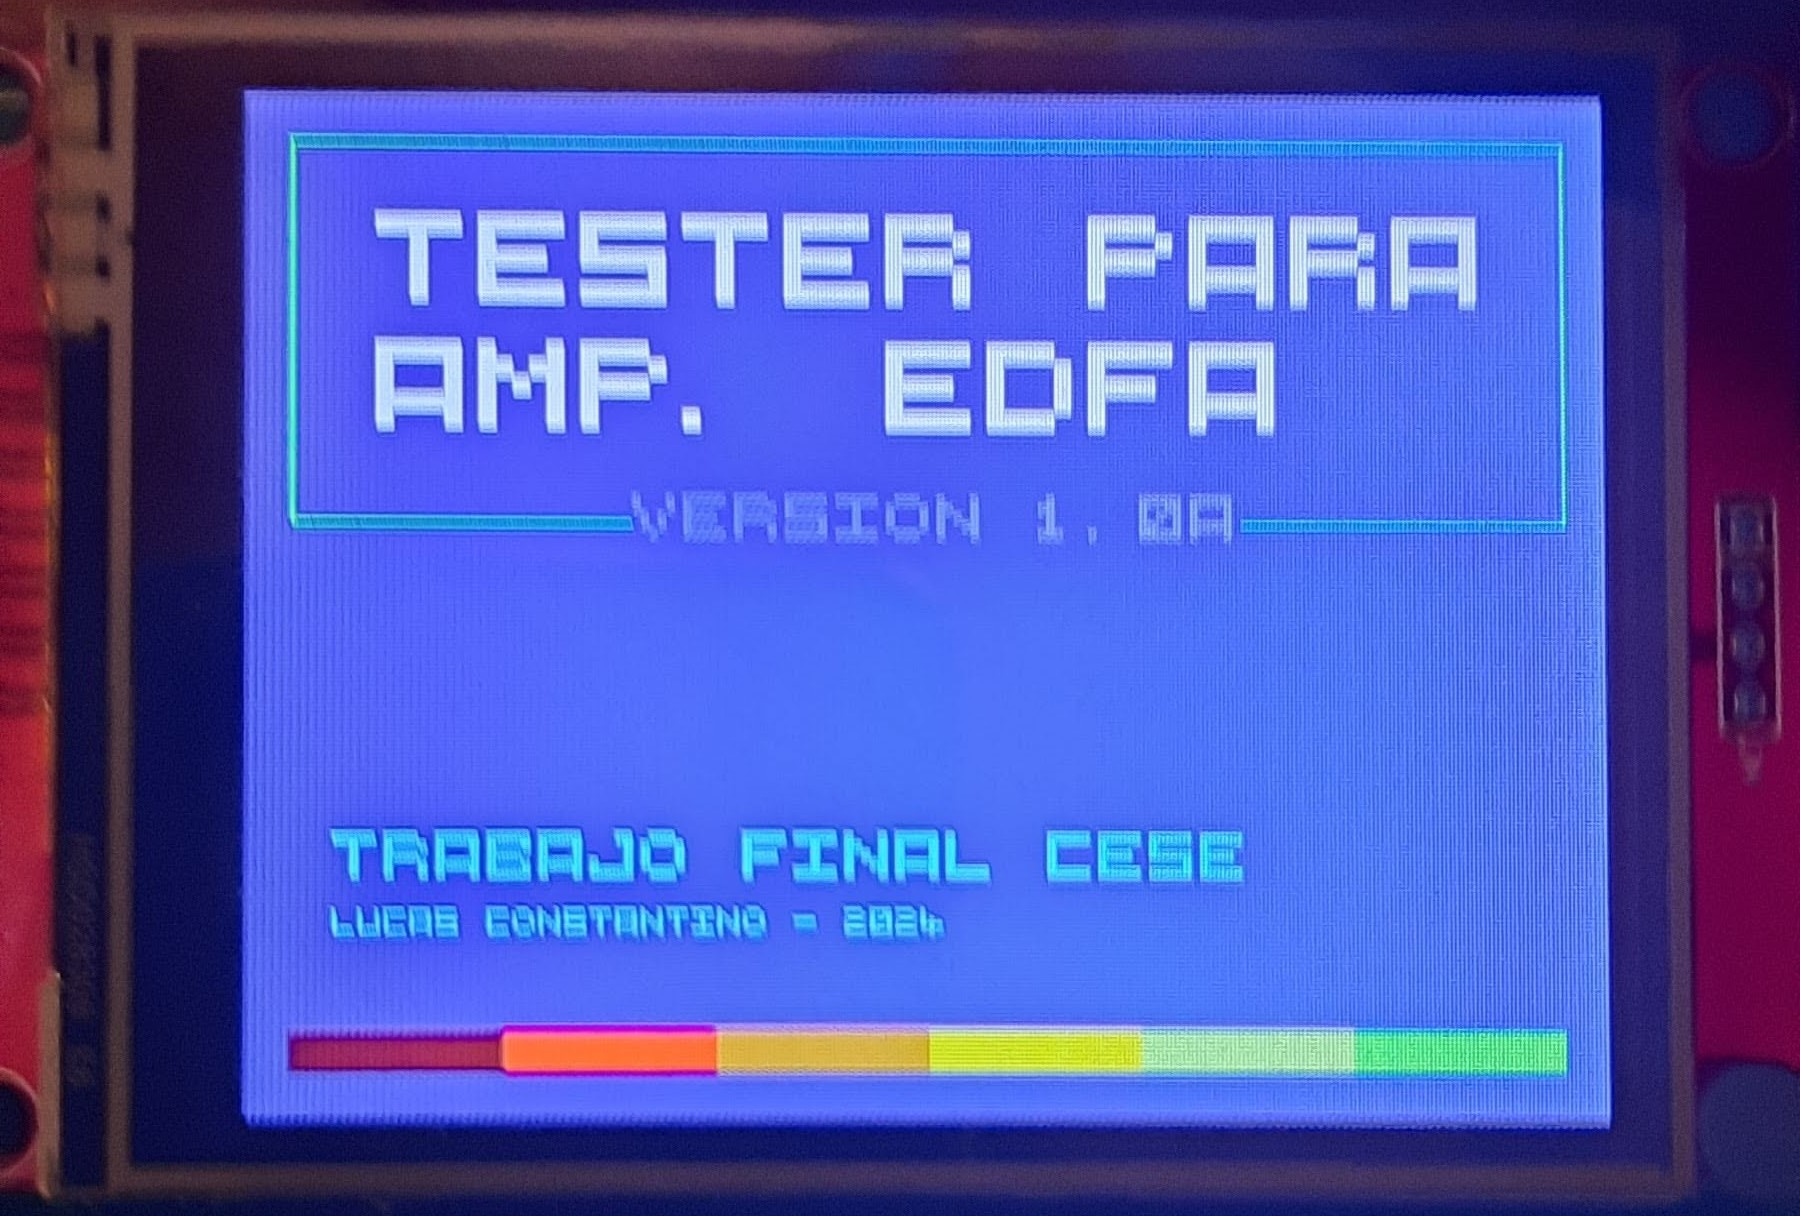
\includegraphics[width=0.8\textwidth]{./Figures/testLCD.jpg}
\caption{Pantalla LCD durante el encendido de la placa.}
\label{fig:testLCD}
\end{figure}

\subsection{Prueba de la consola de control}

La consola de control se encuentra implementada sobre el driver de la UART por lo que al validar el funcionamiento de esta también se estaría validando el del funcionamiento del driver.

Para ello lo que se hace es, mediante el emulador de puertos PuTTY, enviar mediante UART distintos comandos al microcontrolador y verificar que tienen el efecto deseado en la placa. En la figura \ref{fig:pruebaConsola} se puede ver la terminal luego de la ejecución de varios comandos.

\begin{figure}[H]
\centering
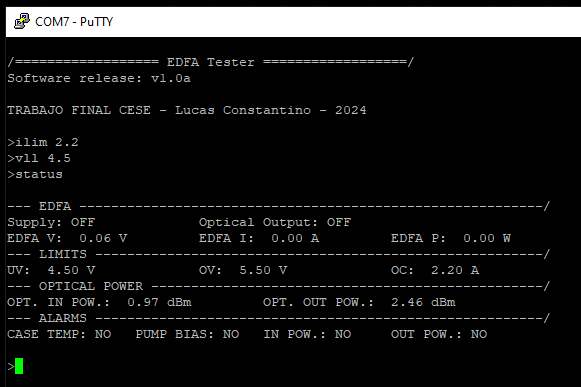
\includegraphics[width=0.9\textwidth]{./Figures/pruebaConsola.png}
\caption{Uso de la consola de control.}
\label{fig:pruebaConsola}
\end{figure}

\section{Pruebas de integración}
\label{sec:pruebasInt}

Las pruebas de integración tienen como objetivo verificar el cumplimiento de los requerimientos establecidos en el documento \citep{DOC_REQ} y mencionados en la sección \ref{sec:reqs}. Al hacer esto se valida la correcta interacción entre el hardware y el firmware, es decir, el funcionamiento del sistema como una unidad.

\subsection{Funcionamiento normal}

En la figura \ref{fig:funcNorm} se puede ver el estado de la pantalla LCD durante el funcionamiento normal, con el amplificador alimentado, su salida óptica prendida y ninguna alarma activa.

\begin{figure}[H]
\centering
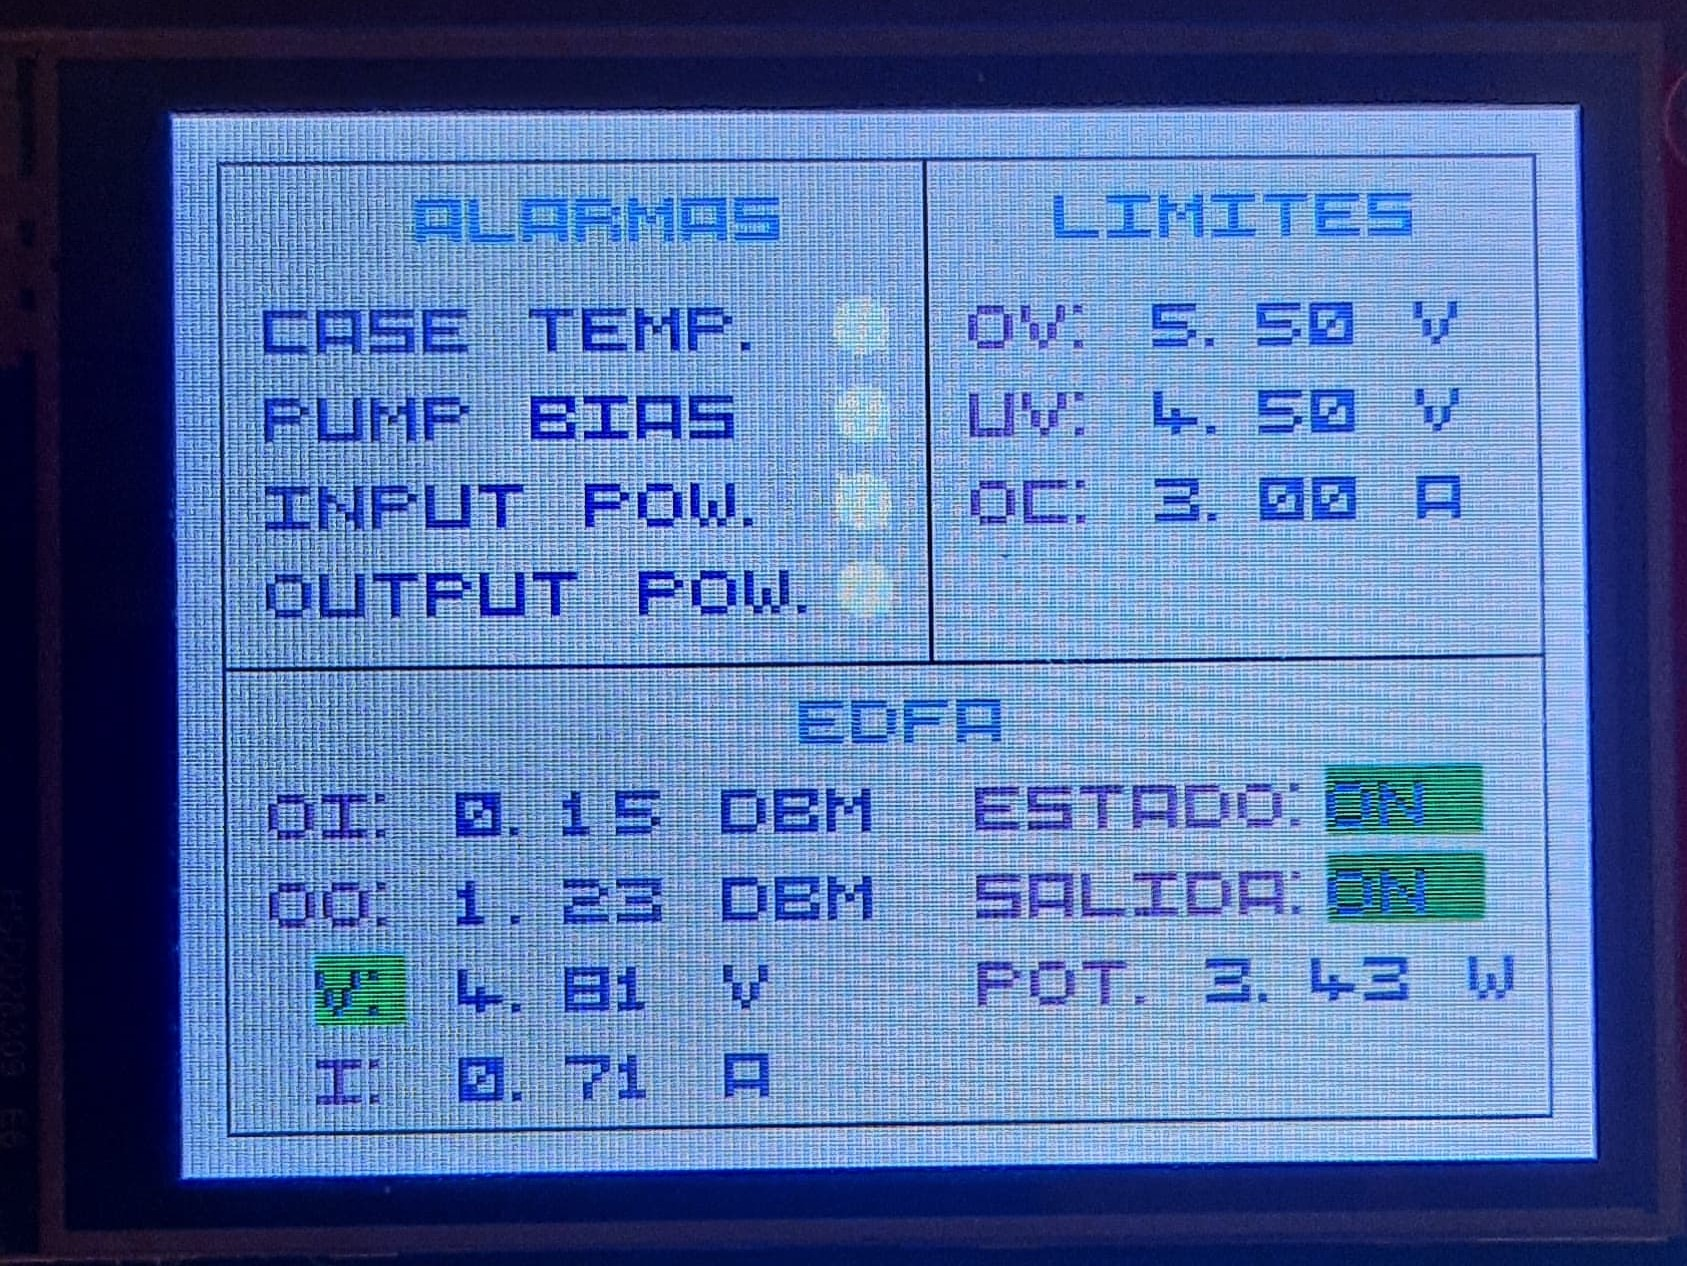
\includegraphics[width=0.75\textwidth]{./Figures/funcNorm.jpg}
\caption{Pantalla LCD durante funcionamiento normal.}
\label{fig:funcNorm}
\end{figure}

De aquí se observa que los valores límites, las alarmas y las variables medidas se actualizan con la frecuencia pretendida en el programa.

\subsection{Detección de alarmas}

Cuando alguna de las alarmas se activa mientras la salida óptica del amplificador permanece encendida, esta se debe apagar inmediatamente mediante la señal de control OUT\_POW\_MUTE, ya que de no hacerlo, esto podría dañar el EDFA.

En la figura \ref{fig:detecAlarm2} se puede ver la conmutación de la señal de control OUT\_POW\_MUTE (canal D1 en rojo) cuando la señal de alarma CASE\_TEMP\_ALARM se activa (canal D0 en blanco). Ambas señales son activas en nivel alto.

\begin{figure}[H]
\centering
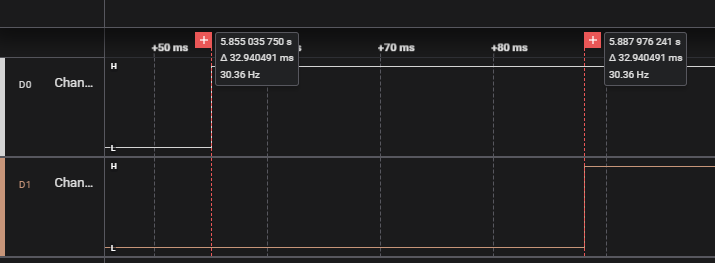
\includegraphics[width=1\textwidth]{./Figures/detecAlarm2.png}
\caption{Detección de alarma y apagado de salida óptica.}
\label{fig:detecAlarm2}
\end{figure}

En la figura anterior se puede observar que el tiempo de retardo que existe entre la detección de la alarma del EDFA y el apagado de la salida óptica es de aproximadamente 33 ms, valor que cumple con el requerimiento 4.2 especificado en la sección \ref{sec:reqs}.

En la figura \ref{fig:detecAlarm} se puede ver el estado de la pantalla LCD luego de la detección de la alarma. El amplificador permanece alimentado pero su salida apagada.

\begin{figure}[H]
\centering
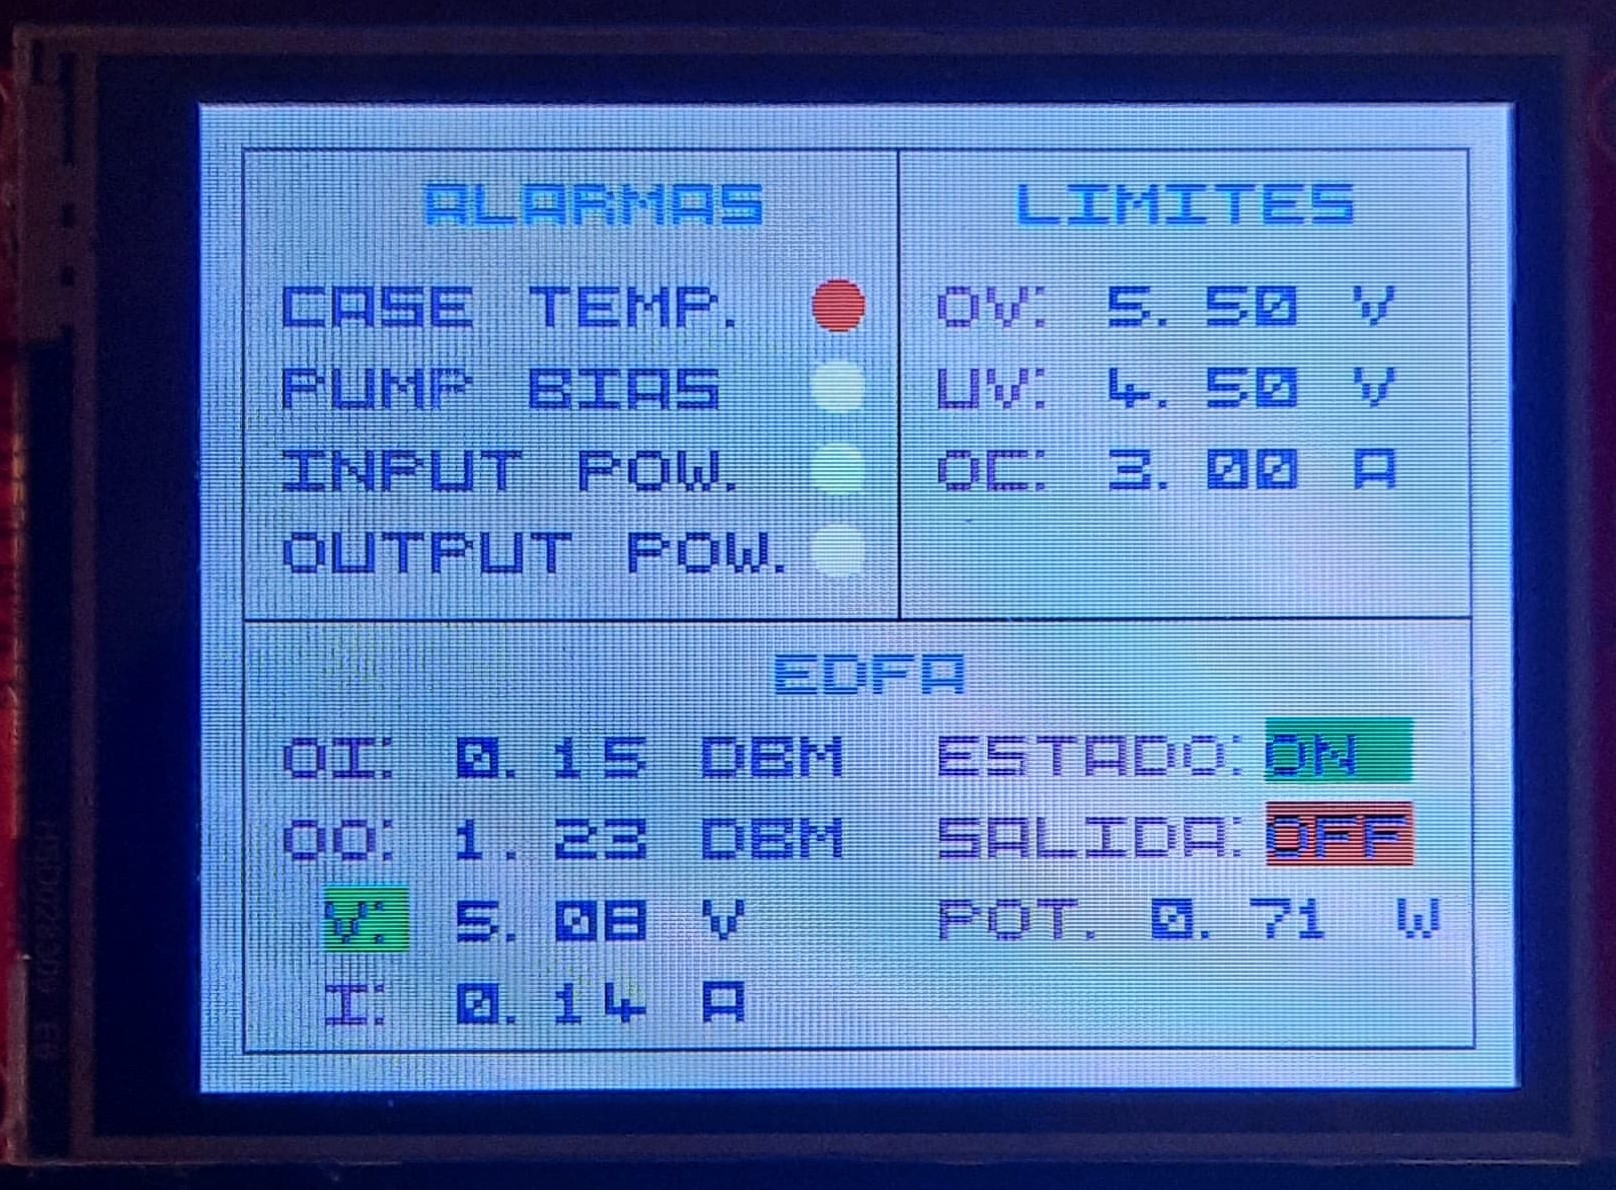
\includegraphics[width=0.75\textwidth]{./Figures/detecAlarm.jpg}
\caption{Pantalla LCD luego de detección de alarma.}
\label{fig:detecAlarm}
\end{figure}

\subsection{Detección de sobrecorriente}

Al igual que para el caso de la detección de alarmas, la detección de una sobrecorriente también debe procesarse rápidamente. En este caso, se asoció la señal de alarma del monitor de corriente a una interrupción en el programa, y se midió el retardo entre el momento en que se activa dicha señal y la desactivación de la señal que controla el relé de alimentación.

En la figura \ref{fig:detecOC} se puede ver la conmutación de la señal que controla la activación del relé (canal D1 en rojo) luego de que la señal de alarma del monitor de corriente se activa (canal D0 en blanco). En este caso la alarma es activa en nivel bajo.

\begin{figure}[H]
\centering
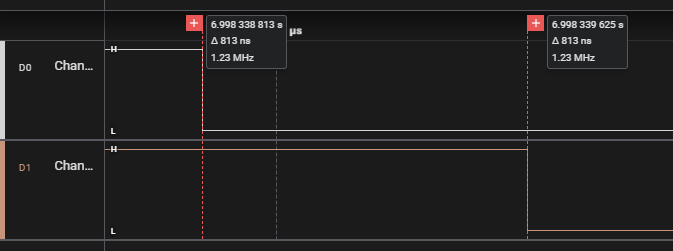
\includegraphics[width=1\textwidth]{./Figures/detecOC.png}
\caption{Detección de sobrecorriente y desconexión del EDFA.}
\label{fig:detecOC}
\end{figure}

Se puede observar que el tiempo de retardo que existe entre la detección de la sobrecorriente y la desconexión del relé es menor a 1~\textmu s, valor que cumple holgadamente con el requerimiento 4.1 especificado en la sección \ref{sec:reqs}.

\section{Comparación del prototipo con el producto existente}

En la tabla \ref{tab:comparacionDisp} se puede ver una comparación entre las funcionalidades del producto existente y las del prototipo desarollado en este trabajo.

\begin{table}[H]
	\centering
	\caption{Comparación entre el dispositivo implementado y el existente.}
	\begin{tabular}{p{6cm} c c}
		\toprule
		\textbf{Característica} & \textbf{Producto existente} & \textbf{Dispositivo desarrollado} \\
		\midrule
		Interfaz UART	& Sí	& Sí \\
		Testigo de alarmas	& Sí	& Sí \\
		Llaves para señales de control		& Sí	& Sí \\
		Alimentación de EDFA				& Sí	& Sí \\
		Detección de sobrecorriente	& No & Sí \\
		Detección de sobretensión		& No & Sí \\
		Detección de baja tensión		& No & Sí \\
		Protección de potencia óptica de entrada	& No & Sí \\
		Protección de potencia óptica de salida		& No & Sí \\
		Desconexión automática de EDFA en caso de alarma & No & Sí \\
		Protección contra descarga electrostática en pines & No & Sí \\
		\bottomrule
		\hline
	\end{tabular}
	\label{tab:comparacionDisp}
\end{table}

\section{Cumplimiento de requerimientos}


% Chapter Template

\chapter{Conclusiones} % Main chapter title

\label{Chapter5} % Change X to a consecutive number; for referencing this chapter elsewhere, use \ref{ChapterX}


%----------------------------------------------------------------------------------------
%	Chapter 5
%----------------------------------------------------------------------------------------

El último capítulo resume los resultados alcanzados en este trabajo, el grado de cumplimiento de los requerimientos y plantea las mejoras necesarias en etapas futuras.

\section{Conclusiones generales}

En líneas generales, a pesar de los contratiempos encontrados durante el desarrollo, el trabajo se llevó a cabo con éxito ya que:  

\begin{itemize}
\item Se obtuvo un prototipo validado del hardware, lo que permite volver a usar el mismo diseño y componentes en el producto final.
\item Se desarrolló una primera versión validada del firmware.
\item Se logró interiorizarse en la tecnología de los EDFA y su funcionamiento.
\item Como se explica en la sección \ref{sec:dispImp}, el dispositivo desarrollado no es el producto final si no una primera versión que funciona como prueba de concepto y simulador del comportamiento del amplificador. Aún así, logra cumplir con los requerimientos principales establecidos por la empresa, lo que permite darlo por finalizado y pasar a la etapa de desarrollo del producto final.
\item Se hizo uso de muchas herramientas, conceptos y metodologías incorporadas durante la cursada de la especialización, dando como resultado un trabajo profesional y facilitando su desarrollo.
\end{itemize}

\section{Trabajo futuro}

Con el objetivo de contar con un producto final apto para uso en tareas de integración e investigación y desarrollo, se planea avanzar en varios aspectos. Entre estos se encuentran:

\begin{itemize}
\item El rediseño y la fabricación de la versión final del PCB del tester, corrigiendo los errores de diseño encontrados en el prototipo. También se deberá incluir el microcontrolador de la placa NUCLEO-144 o un equivalente junto con su interfaz de programación. Todo esto se debe hacer teniendo en cuenta su factor de forma ya que se deberá conectar a un EDFA y montarse sobre una carcasa. 
\item Mejorar el firmware añadiendo más funcionalidades y robustecerlo corrigiendo errores.
\item Una vez rediseñado el PCB, volver a validar el hardware y firmware utilizando un EDFA provisto por la empresa.
\item Realizar las modificaciones necesarias en el firmware para lograr compatibilidad con los \textit{scripts} de Python que la empresa utiliza para ejecutar pruebas de aceptación y funcionamiento automatizadas.
\end{itemize}

%----------------------------------------------------------------------------------------
% Apéndices
%----------------------------------------------------------------------------------------

\appendix

% Incluir apéndices desde archivos separados si es necesario
\begin{landscape}

% Appendix A

\chapter{Circuito esquemático completo} % Main appendix title

\label{AppendixA} % For referencing this appendix elsewhere, use \ref{AppendixA}

A continuación se puede ver el circuito esquemático completo del dispositivo fabricado y ensamblado.

\begin{figure}[H]
\centering
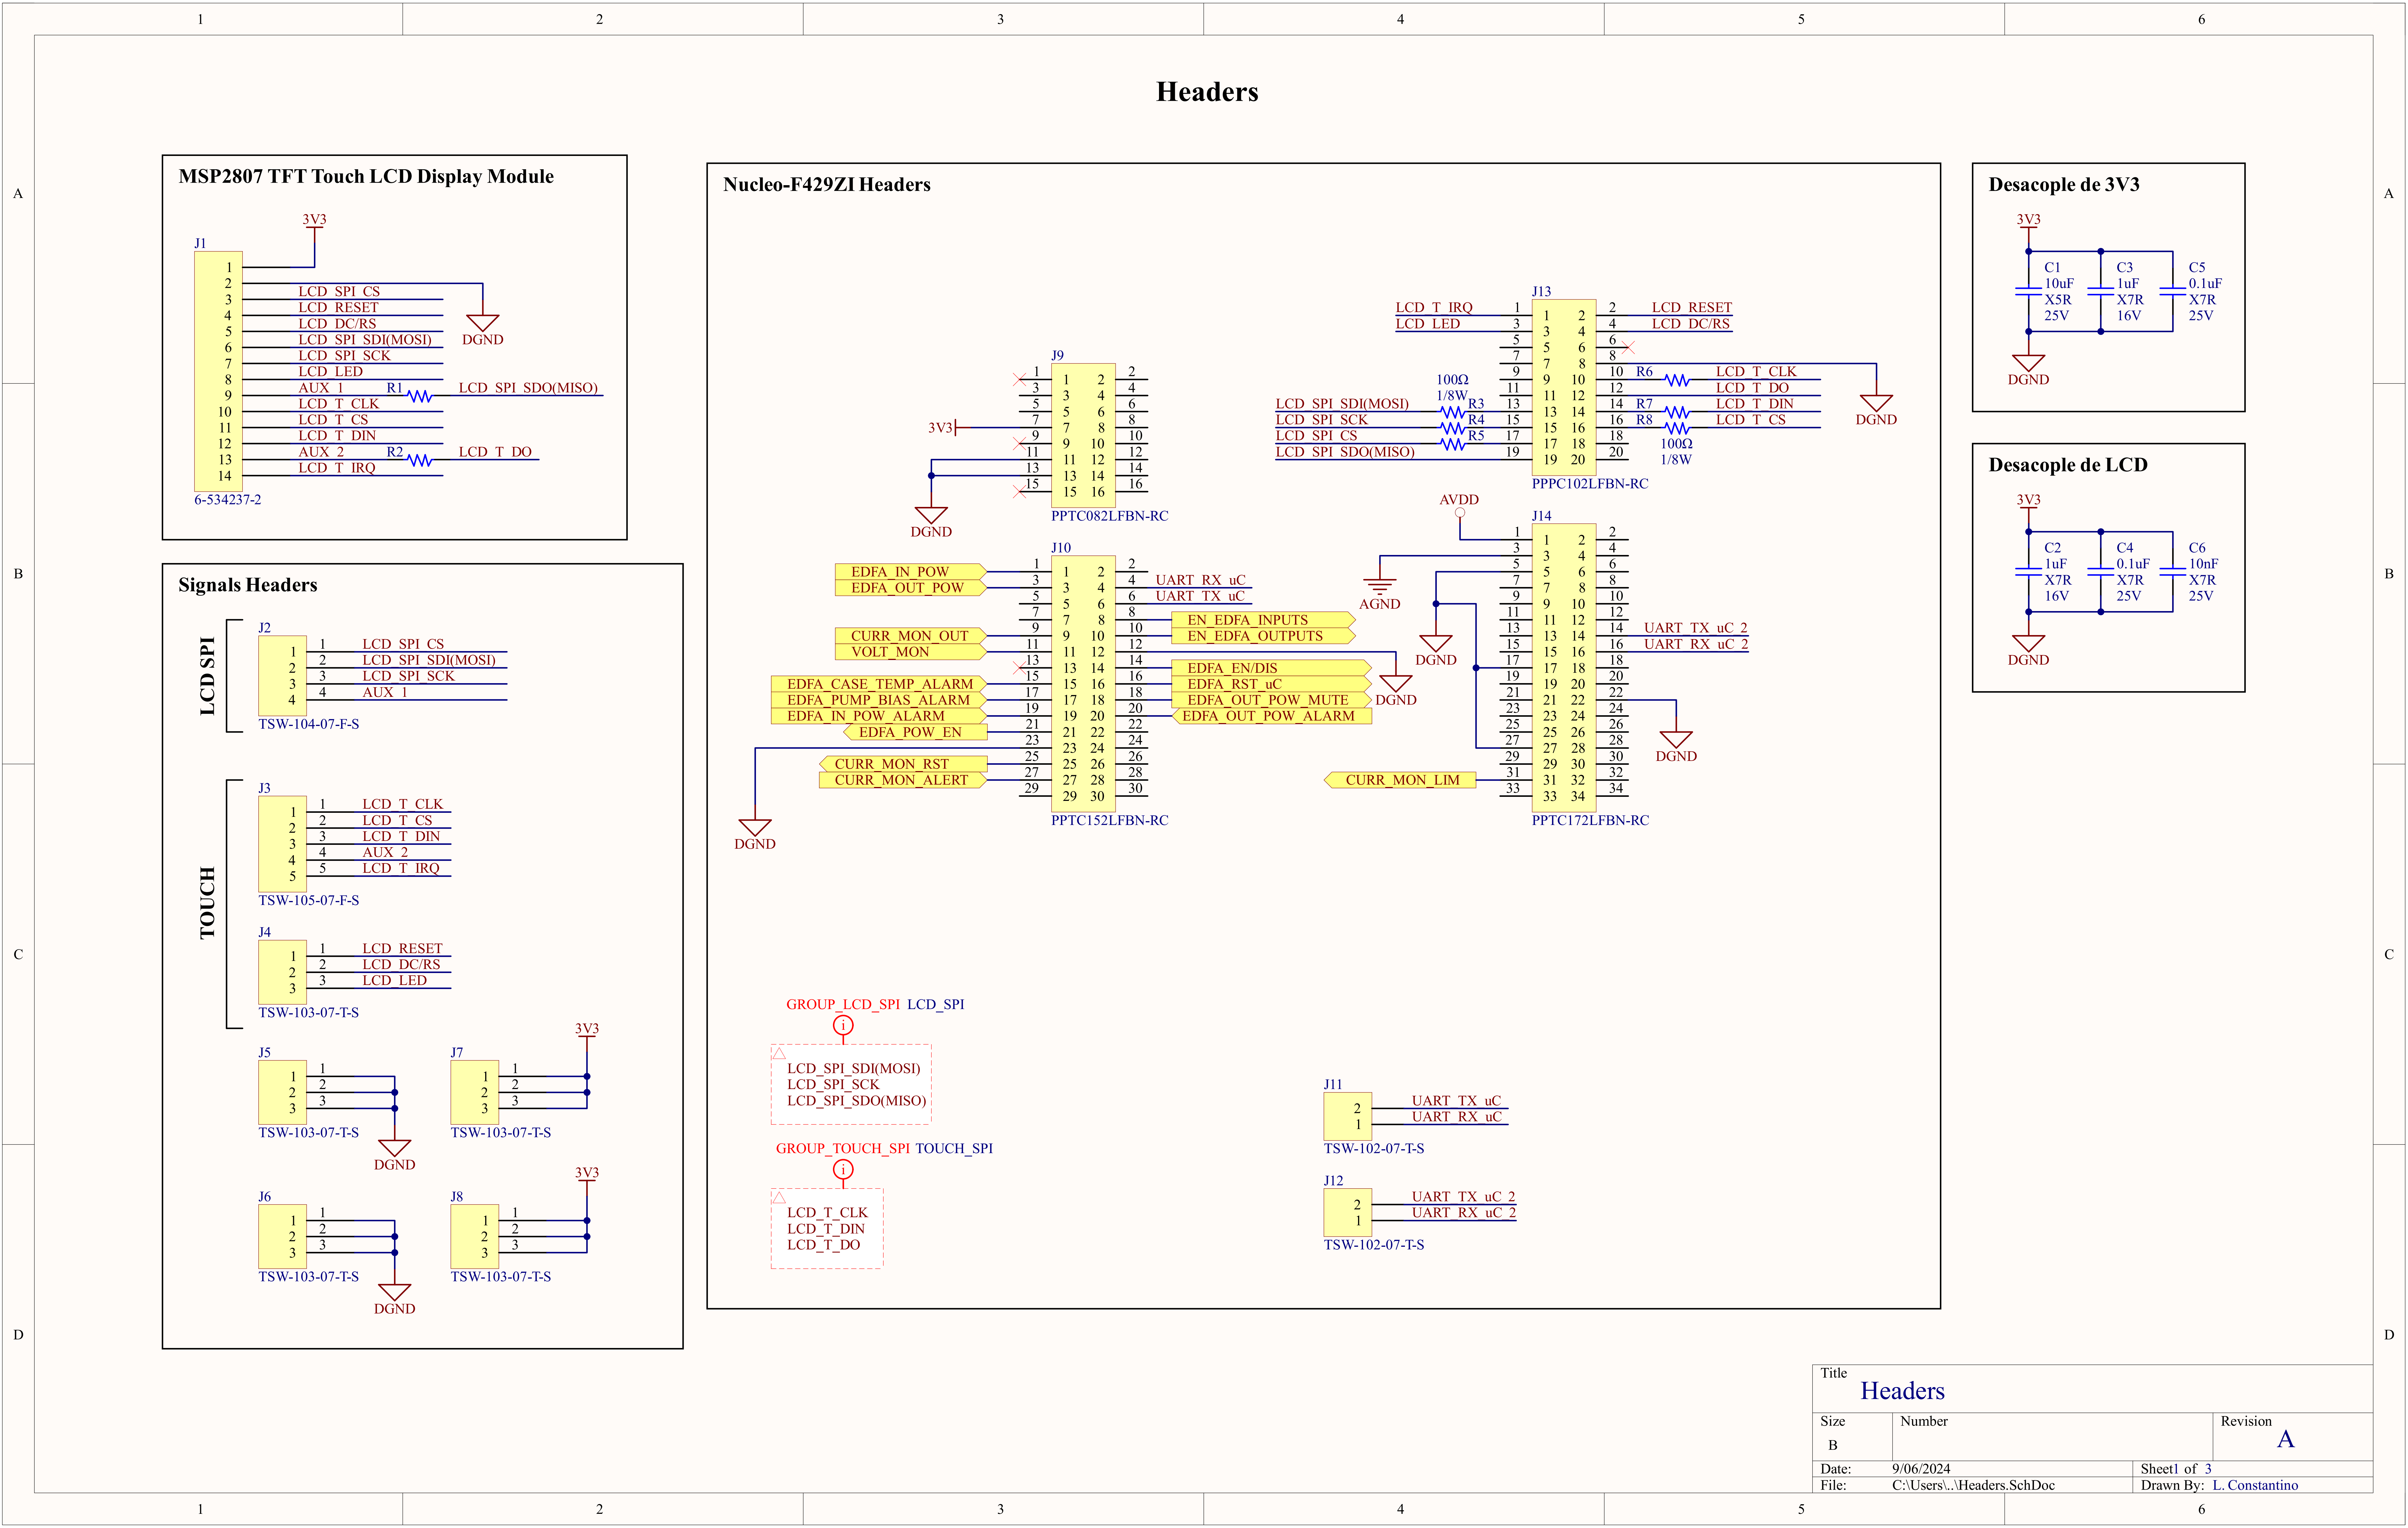
\includegraphics[width=1.7\textwidth]{./Figures/circ1.png}
\caption{Circuito esquemático. Conectores.}
\end{figure}

\begin{figure}[H]
\centering
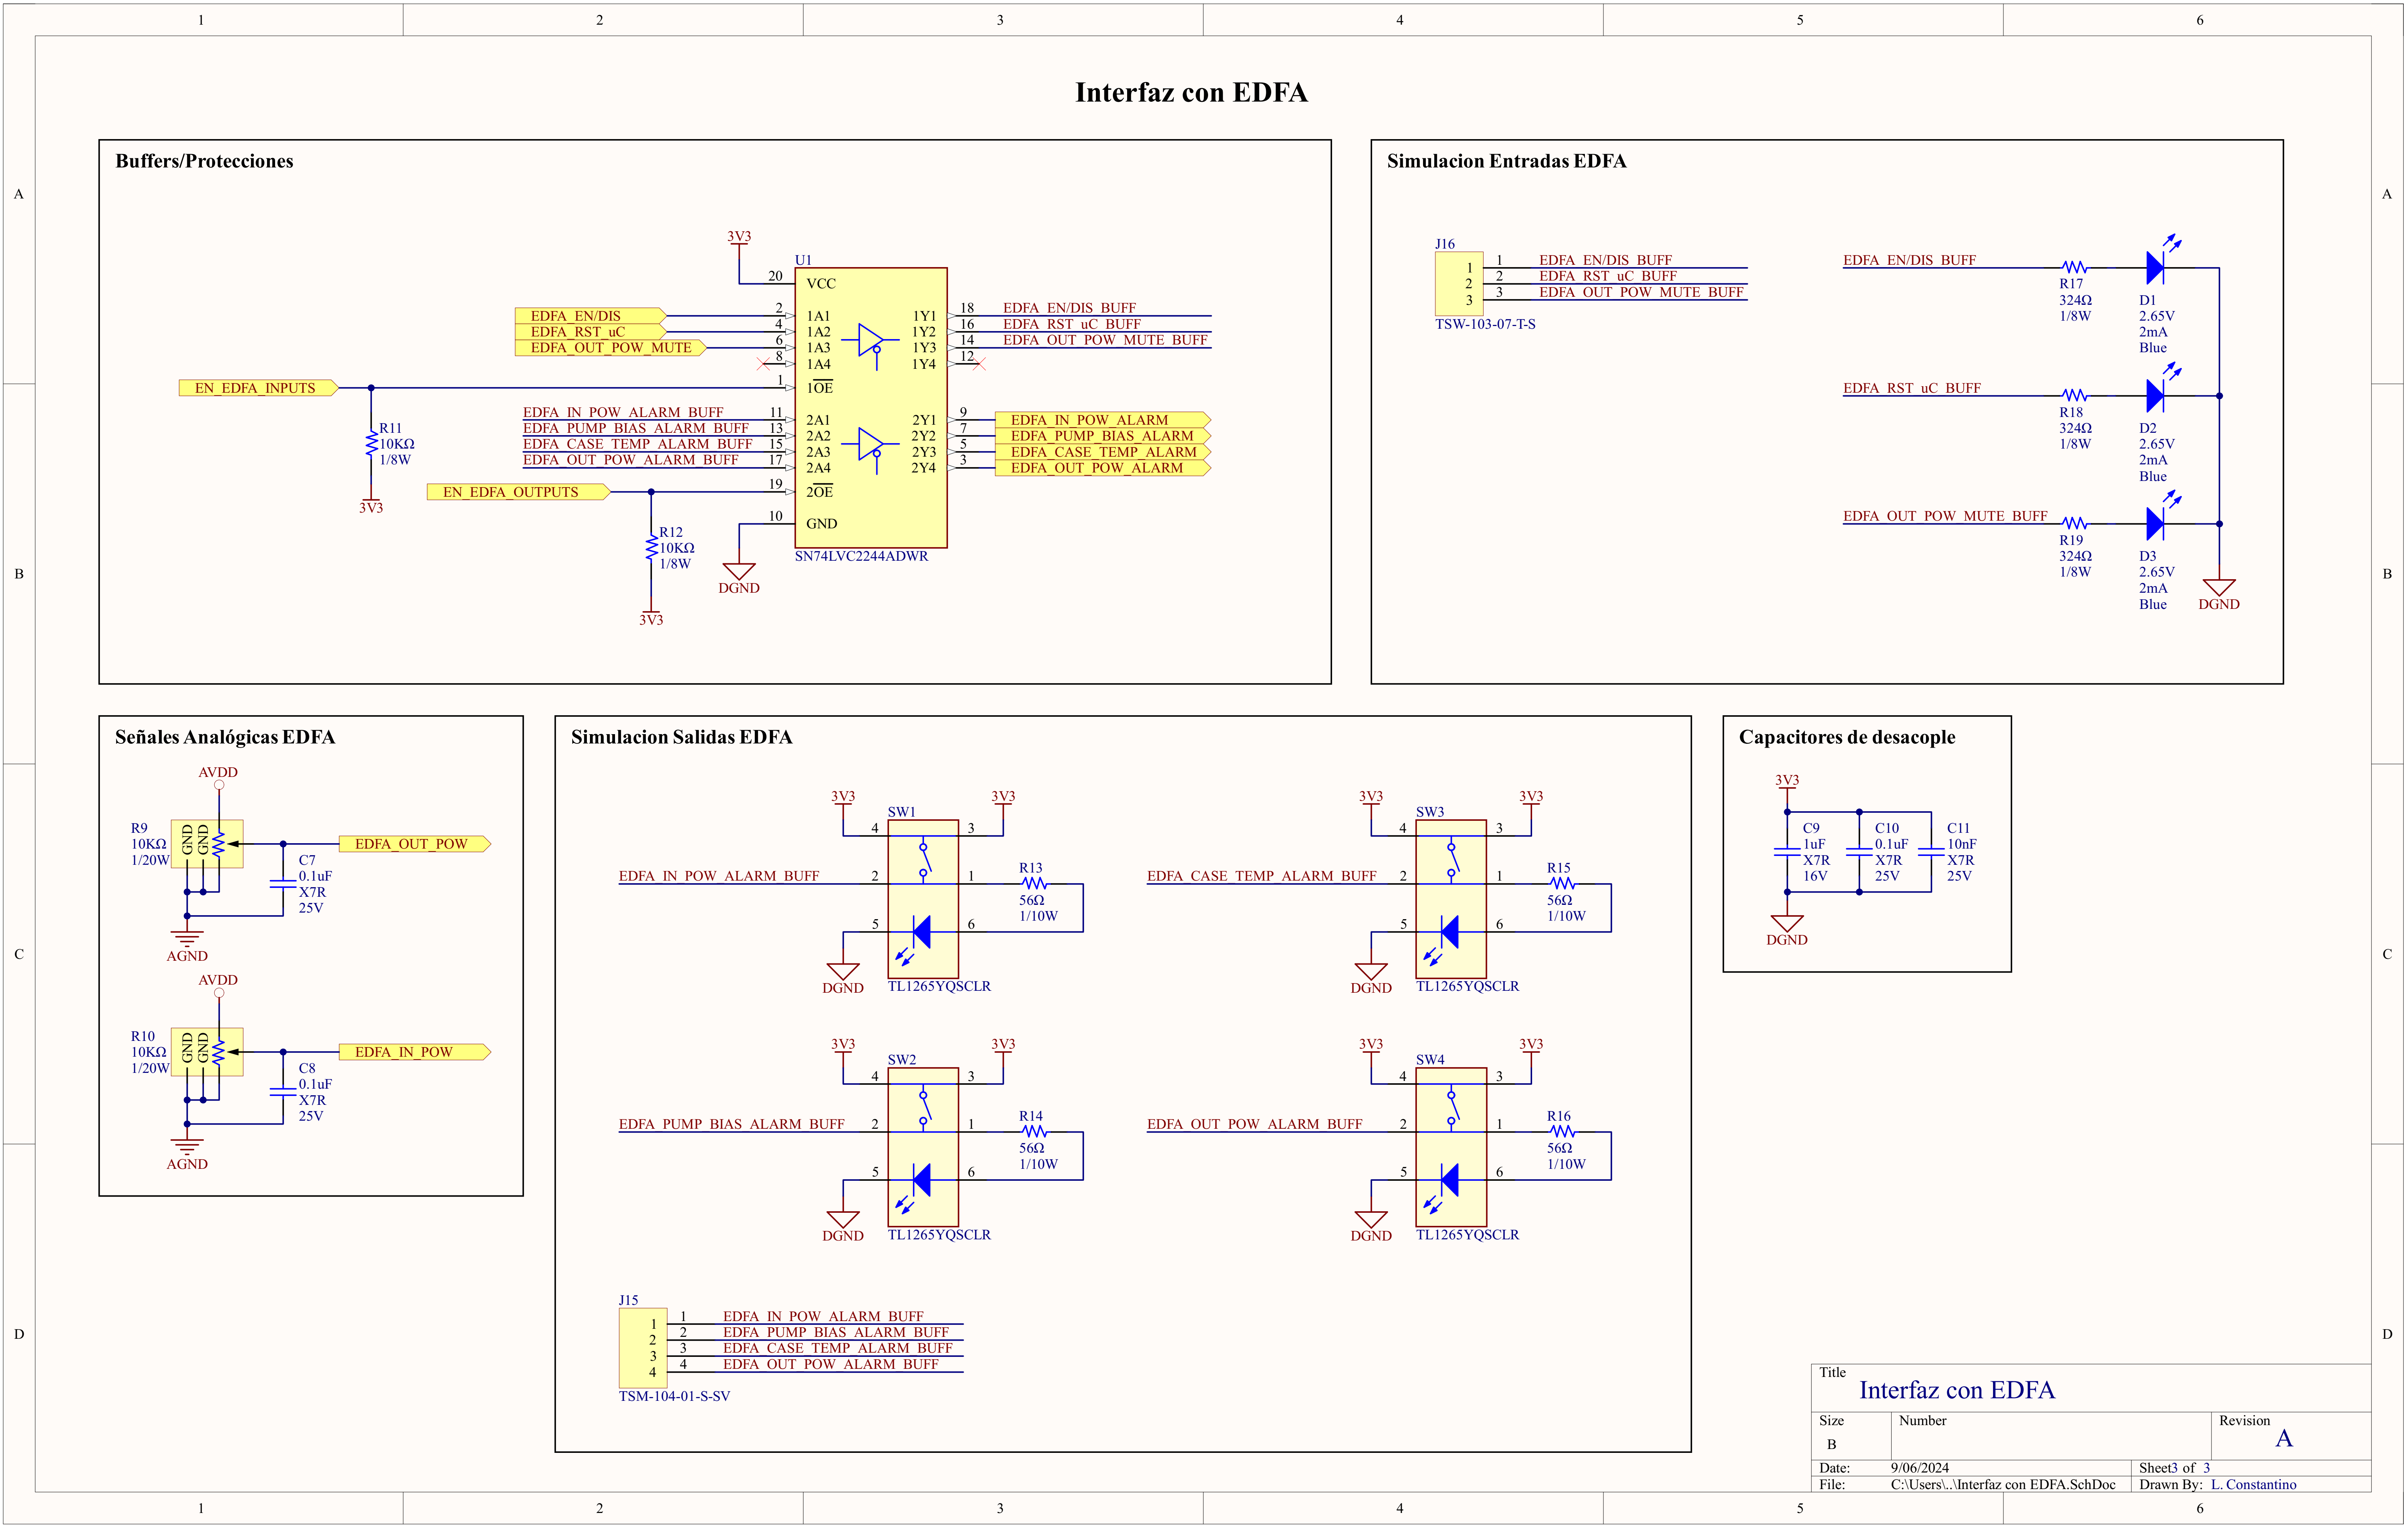
\includegraphics[width=1.7\textwidth]{./Figures/circ2.png}
\caption{Circuito esquemático. Interfaz con EDFA.}
\end{figure}

\begin{figure}[H]
\centering
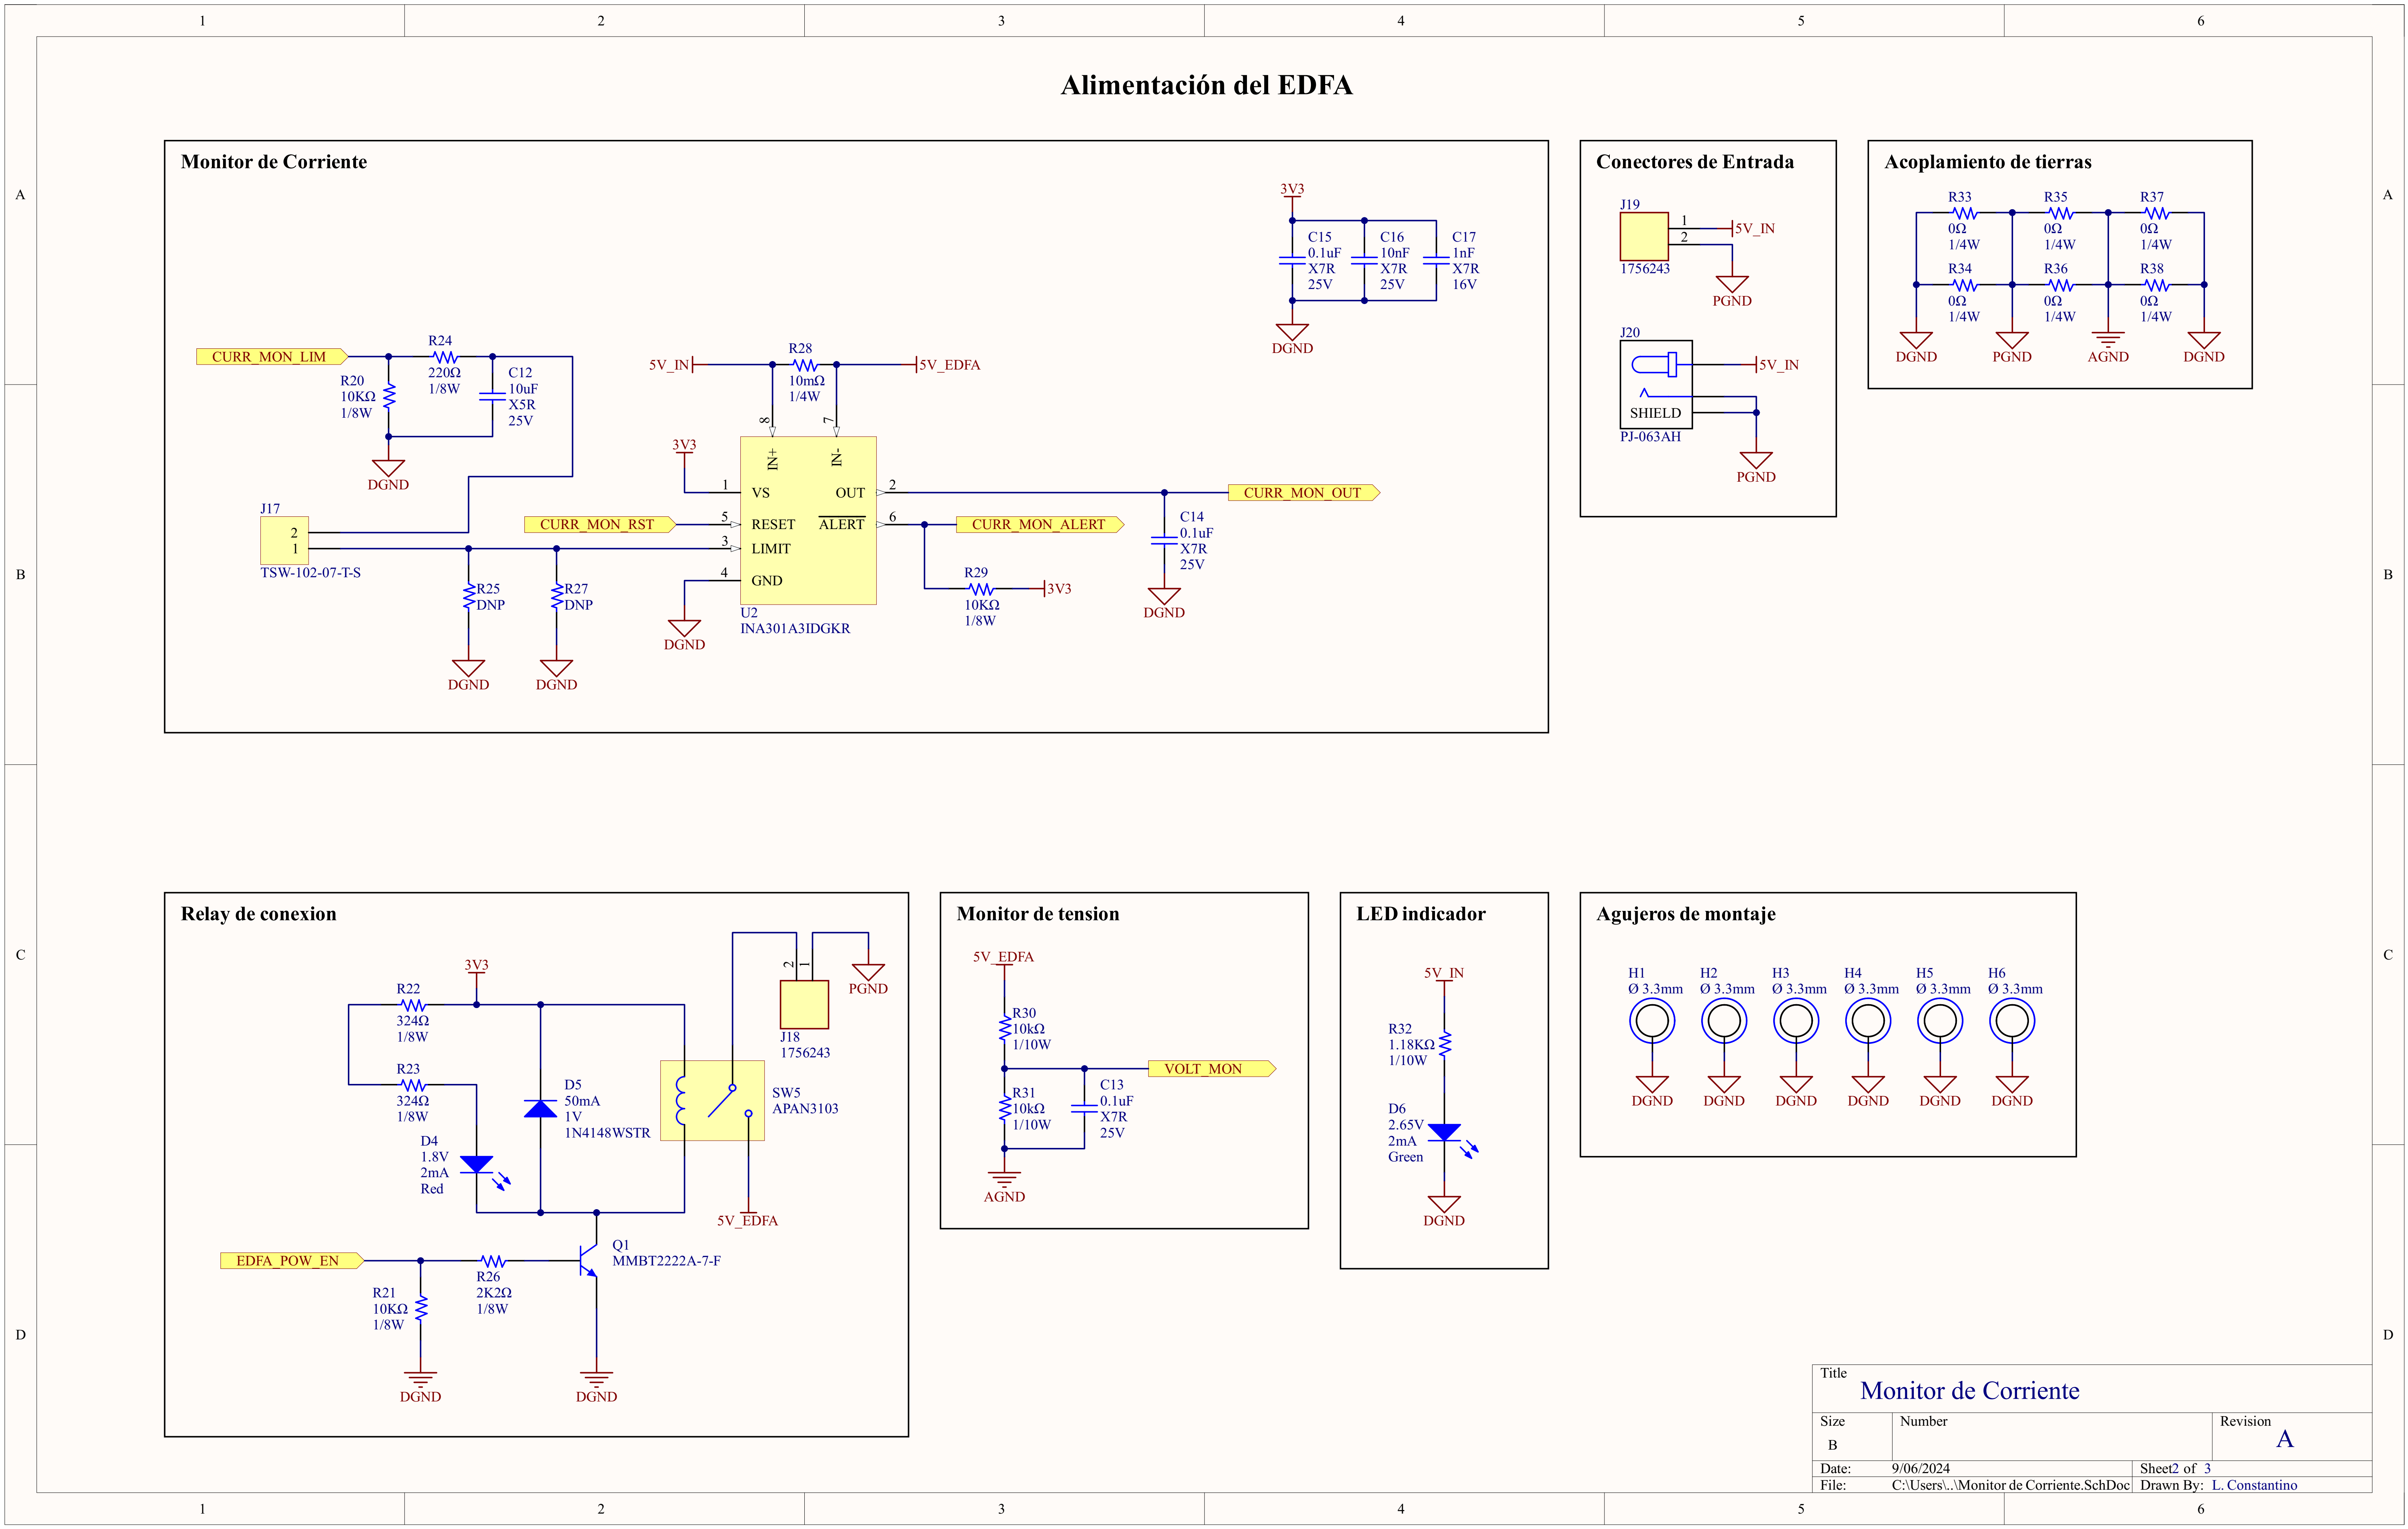
\includegraphics[width=1.7\textwidth]{./Figures/circ3.png}
\caption{Circuito esquemático. Alimentación del EDFA.}
\end{figure}

\end{landscape}

% Appendix A

\chapter{Banco de ensayos} % Main appendix title

\label{AppendixB} % For referencing this appendix elsewhere, use \ref{AppendixA}

A continuación se puede ver el banco de ensayos con todos los instrumentos y componentes necesarios para ejecutar las pruebas de hardware y firmware.

\begin{figure}[H]
\centering
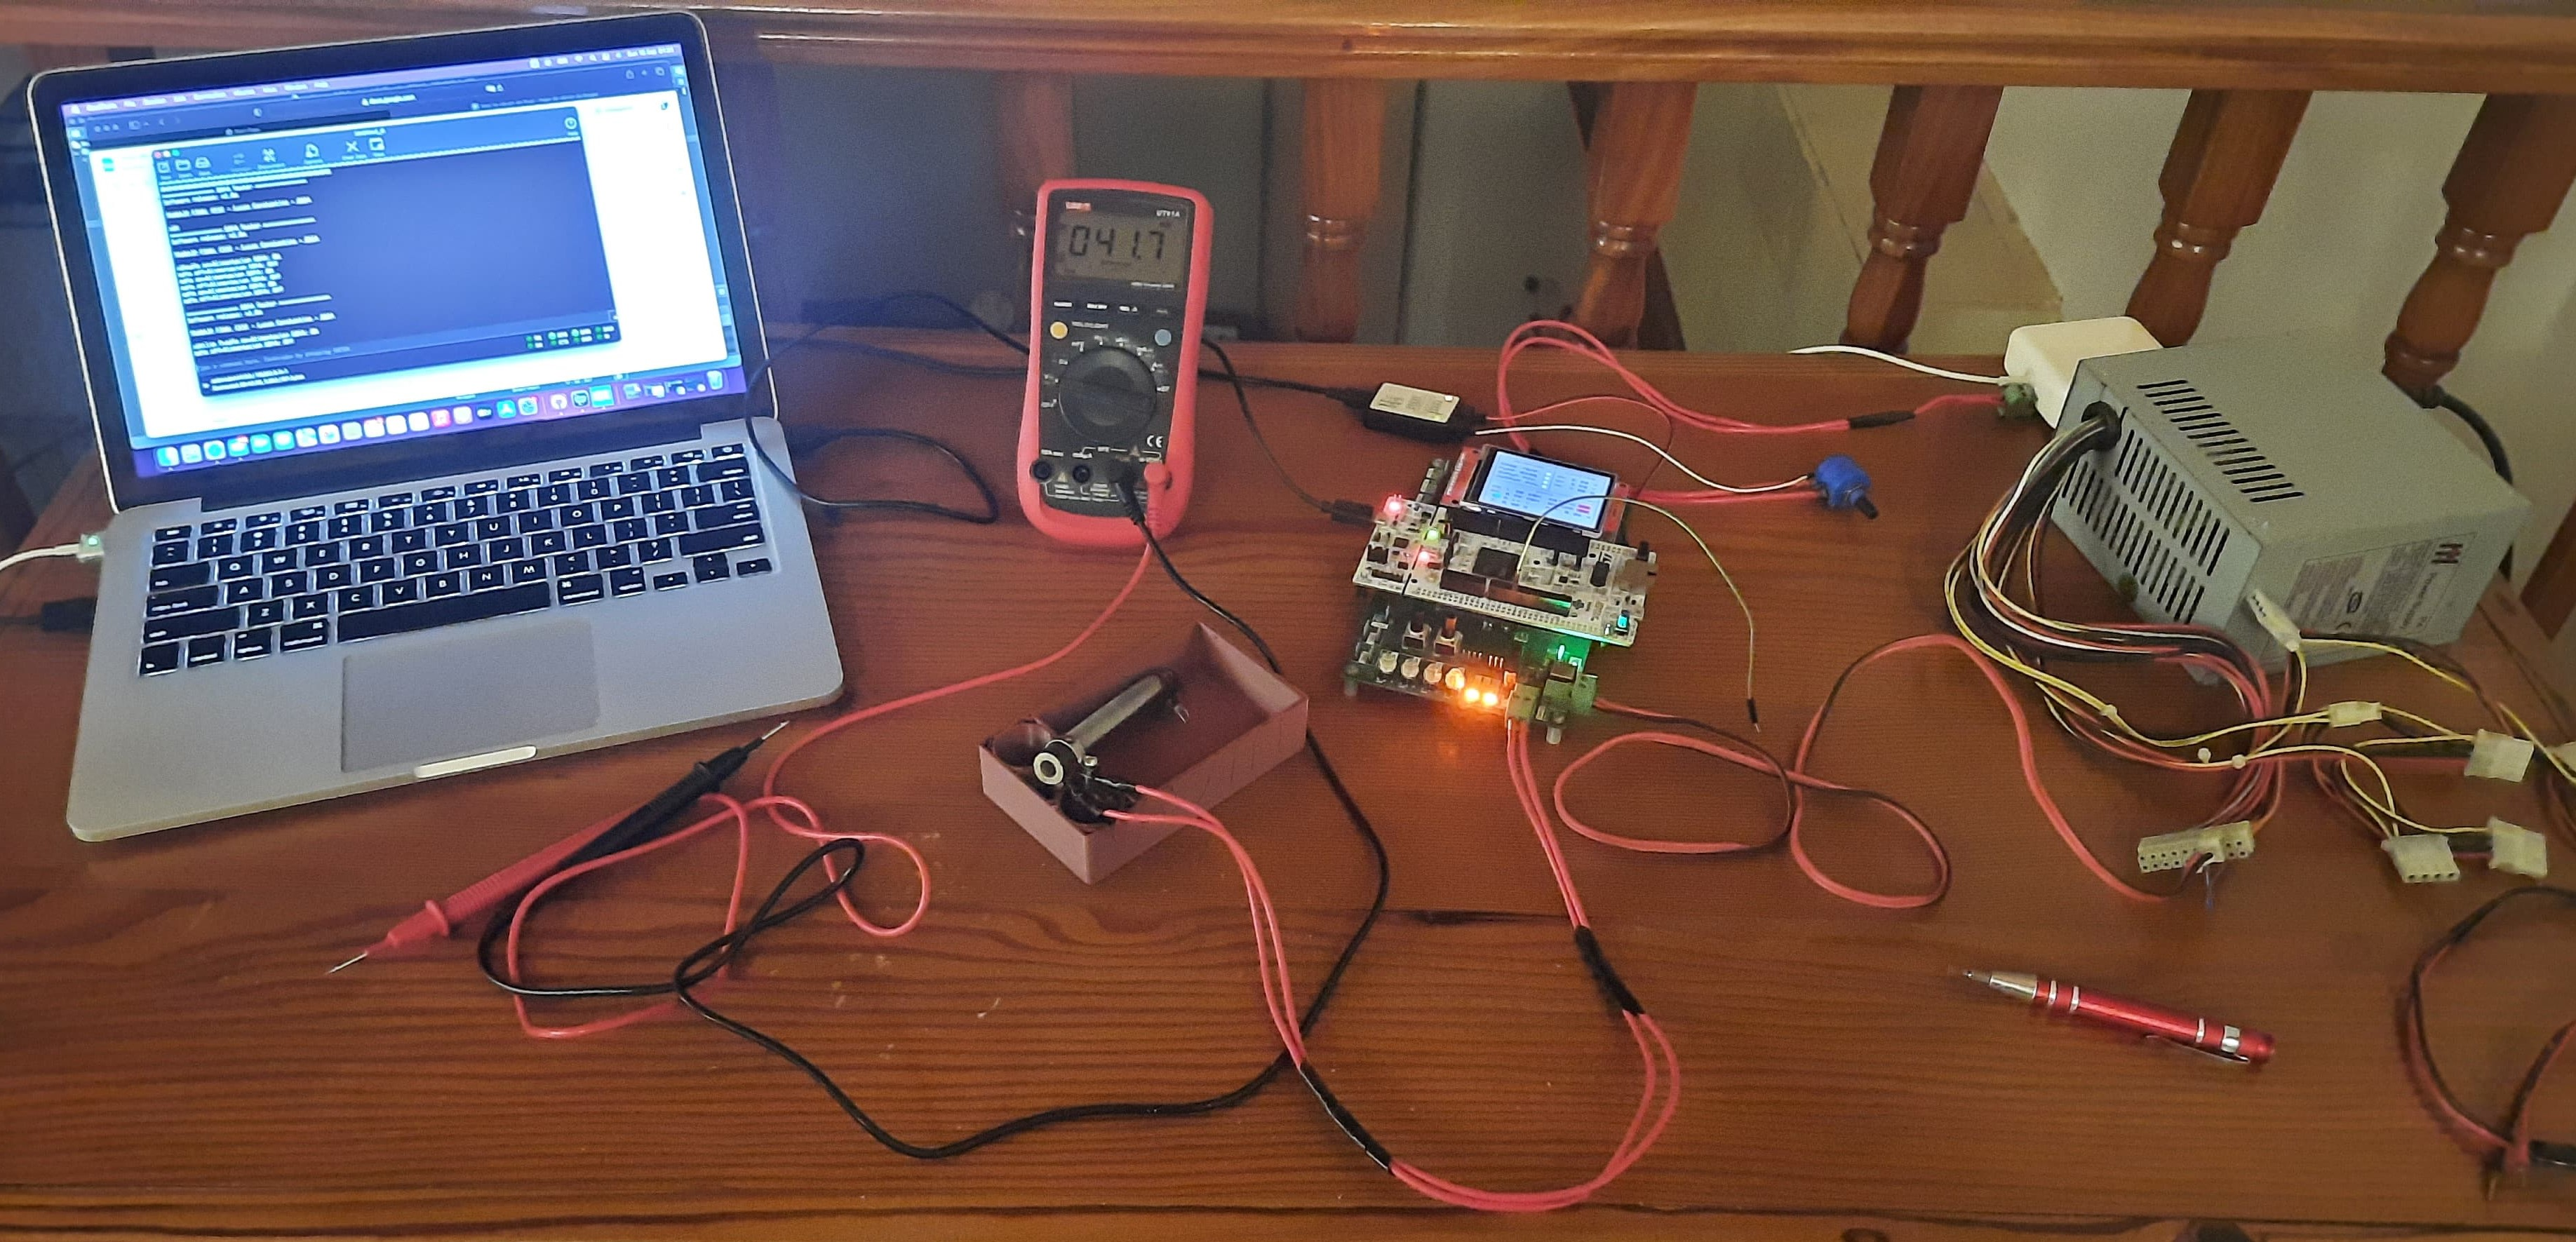
\includegraphics[width=1\textwidth]{./Figures/setupEnsayos.jpg}
\caption{Banco de ensayos.}
\label{fig:setupEnsayos}
\end{figure}

%----------------------------------------------------------------------------------------
% Bibliografía
%----------------------------------------------------------------------------------------

\renewcommand{\bibname}{Bibliografía} % Para asegurarte de que el título sea correcto
\phantomsection % Necesario para que el enlace del marcador sea correcto

\printbibliography[heading=bibintoc]

\end{document}






